\documentclass[utf8]{beamer}
\usepackage{etex}
%%%%%%%%%%%%%%%%%%%%%%%%%%%%%%%%%%%%%%%%%%%%%%%%%%%%%%%%%%%%%%%%%%%%%%%%%%
% There are a number of symbols (e.g., \Square) that are defined by      %
% multiple packages.  In order to typeset all the variants in this       %
% document, we have to give glyph a unique name.  To do that, we define  %
% \savesymbol{XXX}, which renames a symbol from \XXX to \origXXX, and    %
% \restoresymbols{yyy}{XXX}, which renames \origXXX back to \XXX and     %
% defines a new command, \yyyXXX, which corresponds to the most recently %
% loaded version of \XXX.                                                %
%                                                                        %

% Save a symbol that we know is going to get redefined.
\def\savesymbol#1{%
  \expandafter\let\expandafter\origsym\expandafter=\csname#1\endcsname
  \expandafter\let\csname orig#1\endcsname=\origsym
  \expandafter\let\csname#1\endcsname=\relax
}

% Restore a previously saved symbol, and rename the current one.
\def\restoresymbol#1#2{%
  \expandafter\let\expandafter\newsym\expandafter=\csname#2\endcsname
  \expandafter\global\expandafter\let\csname#1#2\endcsname=\newsym
  \expandafter\let\expandafter\origsym\expandafter=\csname orig#2\endcsname
  \expandafter\global\expandafter\let\csname#2\endcsname=\origsym
}

% Rather than create a rat's nest of \if statements, we keep the table
% whole and have each symbol conditionally appear.
\makeatletter
\newcommand{\trysym}[1]{\@ifundefined{#1}{\mbox{\tiny N/A}}{\csname#1\endcsname}}
\makeatother
%                                                                        %
%%%%%%%%%%%%%%%%%%%%%%%%%%%%%%%%%%%%%%%%%%%%%%%%%%%%%%%%%%%%%%%%%%%%%%%%%%

%---- usepackages ----
\usepackage{amscd}
\usepackage{amsmath,amssymb,amsfonts}%,mathrsfs}

\usepackage{CJKutf8}
\usepackage{CJKpunct,CJKspace}
\punctstyle{CCT}
\usepackage{xcolor}
\usepackage{pgf,tikz}
\usepackage{graphicx}
\usepackage{subfigure}
%\usepackage{picins}  % 图片嵌入段落宏包 比如照片
%\usepackage{pstool} % for matlabfrag.m figures
\usepackage[english]{babel}
\usepackage[utf8]{inputenc}
\usepackage{times}
\usepackage[T1]{fontenc}
%\usepackage{booktabs}
% Or whatever. Note that the encoding and the font should match. If T1
% does not look nice, try deleting the line with the fontenc.
\usepackage{hyperref}
	\hypersetup{
		CJKbookmarks=true
		pdfpagemode={FullScreen}
	}
%---- set beamer page size to fit 16:9 or 16:10 screen ----
%---- uncomment next line for 16:9 aspect ratio ---
%\usepackage[orientation=landscape,size=custom,width=17.067,height=9.6,scale=0.5,debug]{beamerposter}
%---- uncomment next line for 16:10 aspect ratio ---
%\usepackage[orientation=landscape,size=custom,width=15.36,height=9.6,scale=0.5,debug]{beamerposter}

%---- 重定义字体、字号命令 ----
	\newcommand{\songti}{\CJKfamily{song}}     % 宋体   (Windows自带simsun.ttf)
	\newcommand{\kaishu}{\CJKfamily{kai}}      % 楷体   (Windows自带simkai.ttf)
	\newcommand{\lishu}{\CJKfamily{li}}
	\newcommand{\bodmtblk}{\CJKfamily{bodonimtblk}}
	% ---- 字号设置 ----
	\newcommand{\chuhao}{\fontsize{42pt}{\baselineskip}\selectfont}
	\newcommand{\xiaochuhao}{\fontsize{36pt}{\baselineskip}\selectfont}
	\newcommand{\yichu}{\fontsize{32pt}{\baselineskip}\selectfont}
	\newcommand{\yihao}{\fontsize{28pt}{\baselineskip}\selectfont}
	\newcommand{\erhao}{\fontsize{21pt}{\baselineskip}\selectfont}
	\newcommand{\xiaoerhao}{\fontsize{18pt}{\baselineskip}\selectfont}
	\newcommand{\sanhao}{\fontsize{15.75pt}{\baselineskip}\selectfont}
	\newcommand{\sihao}{\fontsize{14pt}{\baselineskip}\selectfont}
	\newcommand{\xiaosihao}{\fontsize{12pt}{\baselineskip}\selectfont}
	\newcommand{\wuhao}{\fontsize{10.5pt}{\baselineskip}\selectfont}
	\newcommand{\xiaowuhao}{\fontsize{9pt}{\baselineskip}\selectfont}
	\newcommand{\liuhao}{\fontsize{7.875pt}{\baselineskip}\selectfont}
	\newcommand{\qihao}{\fontsize{5.25pt}{\baselineskip}\selectfont}

\mode<presentation>
{
	%\usetheme{Warsaw}
	\usecolortheme{EmoryBlue} % beaver, crane, wolverine - warm color theme
						% dove - black and white color theme
						% seahorse, shark - nice color theme
						% whale, dolphin - blue color theme, use 'outercolortheme' option for 'chamfered' inner theme
						% thu, EmoryBlue
	\usefonttheme{serif} % serif, structurebold, structuresmallcapsserif, professionalfonts
	\useinnertheme[realshadow]{chamfered}
	%\useinnertheme[realshadow, outercolortheme]{chamfered}
	\useoutertheme[nofootline]{wuerzburg}
	%\useoutertheme[nofootline, shadeframetitlebg]{wuerzburg}% options: glossy, nofootline, shadeframetitlebg
	\setbeamercovered{dynamic}
}

%---- setbeamertemplate ----
	%\setbeamertemplate[infolines theme]{headline}{}
	%\setbeamertemplate{footline}{} % ---- 删除底部信息条 ----
	% --删除底部导航工具栏, 替换为页数 或 logo--
	\usenavigationsymbolstemplate{\vbox{\hfill\structure{
		%\usebeamercolor[bg]{palette secondary}{\normalsize\bodmtblk\bfseries SUNIST}
		
\includegraphics[height=0.3cm]{logo/sunist.pdf}
		%
\includegraphics[height=0.3cm]{logo/sunist-wolverine.pdf}
		%
\includegraphics[height=0.3cm]{logo/sunist-thu.pdf}
		%
\includegraphics[height=0.3cm]{logo/sunist-whale.pdf}
		%\tiny\insertframenumber{} / \inserttotalframenumber
	}\hspace{1ex}\vspace*{1ex}}}
%---- 设置背景渐变色 ----
%	\setbeamertemplate{background canvas}[vertical shading][bottom=structure.fg!15,top=white]
	%\setbeamertemplate{frametitle}[horizontal shading][left=blue, right=black]
%---- pictures dir ----
\graphicspath{{pics/}}

%---- sunist logo ----
	% \pgfdeclareimage[height=0.5cm]{thu}{thu.JPG}
	% \logo{\pgfuseimage{thu}}
	%or
	%\logo{\includegraphics[height=0.3cm]{sunistlogo2.pdf}}

% Delete this, if you do not want the table of contents to pop up at
% the beginning of each subsection:
\AtBeginSubsection[]
{
	\begin{frame}<beamer>
		\frametitle{Outline}
		\tableofcontents[currentsection,currentsubsection]
	\end{frame}
}

% If you wish to uncover everything in a step-wise fashion, uncomment
% the following command:
%\beamerdefaultoverlayspecification{<+->}

%---- includeonlyframes ----
%\includeonlyframes{inclonlyframelabel}

%---- set paragraph skip ----%
\setlength{\parskip}{1ex  plus  0.5ex  minus  0.2ex}

% ---- Change the bullets ----
\useitemizeitemtemplate{%
    \tiny\raise1.5pt\hbox{{$\blacksquare$}}%
}
\usesubitemizeitemtemplate{%
    \tiny\raise1.5pt\hbox{{$\blacklozenge$}}%
}
\usesubsubitemizeitemtemplate{%
    \tiny\raise1.5pt\hbox{{$\blacktriangleright$}}%
}
%\usesubsubsubitemizeitemtemplate{%
%    \tiny\raise1.5pt\hbox{{$\bullet$}}%
%}
% Plot a tiny plasma current graph
% Input:
%   #1 Plot data
%   #2 Mean current
\newcommand{\dataplot}[2]{%
    \begin{tikzpicture}[xscale=0.5, yscale=0.03]
        \begin{scope}[ycomb, yscale=0.5]
        	\draw[densely dotted, thin, black!50] (35,0)--(40,0);
            \draw[densely dotted, thin, black!50] (35,#2)--(40,#2);
            \draw[ultra thin, black!80] plot[smooth] #1;
            \node[above left, scale=0.35] at (35,0) {$0$};
            \node[below left, scale=0.35] at (35,#2) {$#2$};
        \end{scope}
    \end{tikzpicture}%
}

%\pgfdeclarehorizontalshading[frametitle.bg]{beamer@frametitleshade}{1em}{%
%	color(0pt)=(frametitle.bg);
%	color(\paperwidth)=(white)
%}

\newcommand{\thankyoupage}[1]{%
	\begin{frame}
		\begin{centering}
		\begin{beamercolorbox}[sep=3pt,center]{title}
			\usebeamerfont{title}\inserttitle\par%
			\ifx\insertsubtitle\@empty%
			\else%
				\vskip0.25em%
				{\usebeamerfont{subtitle}\usebeamercolor[fg]{subtitle}\insertsubtitle\par}%
			\fi%
		\end{beamercolorbox}%
		\end{centering}
		\vskip2em\par
		\begin{centering}
		\hfill
		\begin{beamercolorbox}[wd=0.8\linewidth,center,rounded=true]{palette secondary}
			\usebeamerfont{title  in  head/foot}
			\huge{#1}
		\end{beamercolorbox}
		\hfill
		\end{centering}
	\end{frame}
}

\newcommand<>{\hover}[3]{\uncover#4{%
	\begin{tikzpicture}[remember picture,overlay]%
		\draw[fill,opacity=0.4] (current page.south west)
			rectangle (current page.north east);
		\node at (current page.center) {%
			\begin{minipage}{{#1}}
			\begin{block}{{#2}}
				{#3}
			\end{block}
			\end{minipage}
		};
	\end{tikzpicture}}
}

\newcommand{\myfootnote}[1]{\footnote{\tiny{{#1}}}}

\newcommand{\backupframebegin}{
     \newcounter{framenumberbeforeappendix}
     \setcounter{framenumberbeforeappendix}{\value{framenumber}}
     \setbeamertemplate{headline}[wuerzburg theme appendix]
     \setbeamertemplate{footline}[wuerzburg theme appendix]
}
\newcommand{\backupframeend}{
   \addtocounter{framenumberbeforeappendix}{-\value{framenumber}}
   \addtocounter{framenumber}{\value{framenumberbeforeappendix}}
   \setbeamertemplate{headline}[wuerzburg theme]
   \setbeamertemplate{footline}[wuerzburg theme]
}

%\input{data/ipdata.txt}

\usepackage{booktabs}%, makecell}
\usepackage{overpic}
\usepackage{multirow}
\usepackage{makecell}
%\usepackage{colortbl}
%\usepackage{transparent}
%\usepackage{fixpauseincludegraphics}

%\setbeamertemplate{background canvas}[vertical shading][bottom=structure.fg!15,top=white]
\setbeamertemplate{background canvas}[vertical shading][bottom=white,top=white]

\AtBeginSection[]
{
  \begin{frame}<beamer>
    \frametitle{提纲}
    \tableofcontents[sections={2-},currentsection,subsectionstyle=show/show/hide]%,sections={2-6}]
  \end{frame}
  \addtocounter{framenumber}{-1}
}

\AtBeginSubsection[]
{
  \begin{frame}<beamer>
    \frametitle{提纲}
    \tableofcontents[sections={2-},currentsection,subsectionstyle=show/shaded/hide]
  \end{frame}
  \addtocounter{framenumber}{-1}
}

\newcommand{\onlineref}[1]{{\scriptsize\texttt{[#1]}}}

%\setbeamerfont{itemize/enumerate body}{font=\bf}

\begin{document}
\begin{CJK*}{UTF8}{kai}

%---- 自定义或重定义环境等,一般用于中文幻灯片 ---
%\newenvironment{dingyi}{definition} %自定义环境
\newcommand{dingyi}[definition]{定义}
\newtheorem{li}{例}
\newenvironment{Definition}{\begin{definition}}{\end{definition}}
\def\theoremname{定理}
\def\defname{定义}
\def\lemmaname{引理}
\def\proofname{证明}
\def\corollaryname{推论}
\def\examplename{例}
\newtheorem{proposition}{命题}
\renewcommand\figurename{\rm 图}
\renewcommand\tablename{\bf 表}


\title[答辩]{SUNIST 等离子体电子温度与密度的\\ 原子发射光谱诊断}

\author[谢会乔]{
\quad
\begin{minipage}{4cm}
    博士生:谢会乔\\
    导\quad 师:高\quad 喆\quad 教授
\end{minipage}
}

\institute[工物系]
{
    清华大学工程物理系
}

\date{2014-06-11}

\frame{\titlepage}

\section*{提纲}
\frame{\frametitle{提纲}\tableofcontents[sections={2-},hideallsubsections]}

%%%%%%%%%%%%%%%%%%%%%%%%%%%%%%%%%%%%%%%%%%%%%%%%%%%%%%%%%%%%%%%%%%%%%%%%%%%%%

\section{引言}

\subsection{课题背景与意义}

\begin{frame}{托卡马克等离子体的 $T_{\rm e}$ 与 $N_{\rm e}$ 诊断}
%    \begin{columns}
%    \column{0.65\textwidth}
    \begin{itemize}
      \item 托卡马克聚变研究已经取得重大进展
        \begin{itemize}
          \item JT-60U 上获得等效 Q 值达 1.25 \onlineref{Fujita T, NF(1999)}
          \item JET 上获得最高 $16.1\,{\rm MW}$ 瞬时功率输出 \onlineref{Keilhacker M, NF(1999)}
        \end{itemize}
      \bigskip
      \item 由诊断技术和工具的进步所伴随
        \begin{itemize}
          \item 越来越高的等离子体温度带来考验
        \end{itemize}
      \bigskip
      \item 非侵入(noninvasive)诊断手段受到重视
        \begin{itemize}
          \item 辐射与粒子测量手段的兴起
          \item 主动测量:射入探测粒子束或激光束
          \item 被动测量:被动接收等离子体的光谱或粒子辐射
        \end{itemize}
    \end{itemize}
%    \column{0.35\textwidth}
%    \begin{center}
%      \begin{overpic}[width=\textwidth]{ProbeVapor121123020-bw.jpg}
%    	\put(1,22){\color{white}{中心柱}}
%    	\put(5,30){\color{white}{$\uparrow$}}
%    	
%    	\put(20,87){\color{white}{等离子体}}
%    	\put(32,80){\color{white}{$\downarrow$}}
%    	
%    	\put(43,58){\color{white}{静电探针}}
%    	\put(67,52){\color{white}{$\downarrow$}}
%    	
%    	\put(43,30){\color{white}{烧蚀亮点}}
%    	\put(60,39){\color{white}{$\uparrow$}}
%  	\end{overpic}
%  		SUNIST 静电探针烧蚀\\
%  		\#121123020
%  	\end{center}
%    \end{columns}
\end{frame}

\begin{frame}{同时确定 $T_{\rm e}$ 与 $N_{\rm e}$ 的等离子体谱线辐射强度比法}
	\begin{itemize}
  		\item 通过对等离子体内的碰撞辐射过程进行建模,获得谱线强度比在 $T_{\rm e}-N_{\rm e}$ 空间内的分布
  		\item 根据谱线比实验测量结果确定电子温度与密度
	\end{itemize}
\vspace*{-2em}
	\begin{center}
		$$
		\frac{I_{\lambda_{ji}}}{I_{\lambda_{qp}}}=	\frac{\epsilon_{ji}T_{\lambda_{ji}}\eta_{\lambda_{ji}}}{\epsilon_{qp}T_{\lambda_{qp}}\eta_{\lambda_{qp}}}
		=\frac{1}{F_R}\frac{T_{\lambda_{ji}}N_jA_{ji}}{T_{\lambda_{qp}}N_qA_{qp}}
		$$
	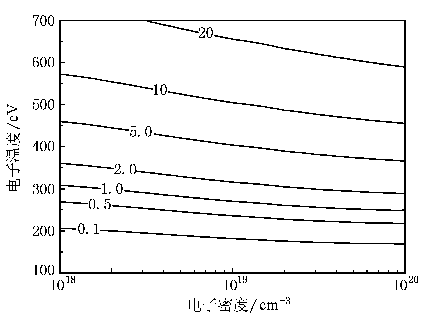
\includegraphics[width=0.33\textwidth]{lijing-a}
	%\hspace*{0.03\textwidth}
	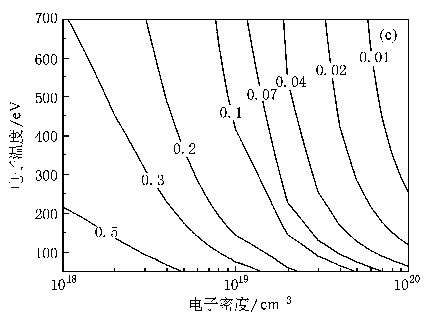
\includegraphics[width=0.33\textwidth]{lijing-b}
	%\hspace*{0.03\textwidth}
	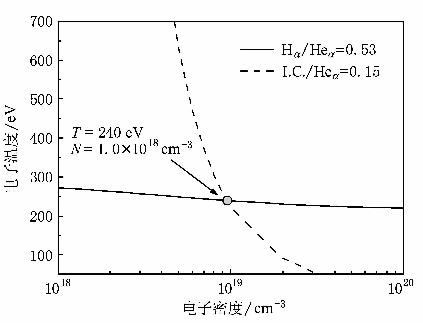
\includegraphics[width=0.33\textwidth]{lijing-c}
	\\
	\hfill\onlineref{Li J. Act.Phys.Sin.(2010)}
	\end{center}
\end{frame}


\begin{frame}{氦原子发射光谱诊断}
	\begin{itemize}
		\item 可见光波段发射光谱诊断
			\begin{itemize}
				\item 测量设备简单、成熟
				\item 不易受复杂电磁场干扰
				\item 少维护/免维护
				\item 容易扩展实现时空分辨测量
			\end{itemize}
		\bigskip
		\item 氦原子发射光谱对聚变等离子体研究具有特殊意义
			\begin{itemize}
				\item 最高的第一电离能:束诊断穿透深度深
				\item 聚变产物:不带来杂质污染
				\item 两套自旋态能级系统:三条谱线的两个谱线比可以同时确定 $T_{\rm e}$ 和 $N_{\rm e}$
			\end{itemize}
	\end{itemize}
\end{frame}


\begin{frame}{氦原子光谱诊断 $T_{\rm e}$ 与 $N_{\rm e}$ 的研究概况}
	\begin{itemize}
		\item 主动:束发射光谱诊断
			\begin{itemize}
				\item 最早包含至 $n=4$ 的碰撞辐射模型 \onlineref{Brosda PhD Thesis(1993)}
				\item 发展到包含众多能级 $n=500$ \onlineref{Burgos PoP(2012)}
				\item 稳态解,不包含 He$^+$ 与 He$^{2+}$
			\end{itemize}
		\bigskip
		\item 被动:氦等离子体光谱诊断\\ \onlineref{Fujimoto JQSRT(1979), Goto JQSRT(2003)}
			\begin{itemize}
				\item 适用于低温和高温等离子体
				\item 包含的原子能级 $n=20$
				\item 添加强磁场效应 等
			\end{itemize}
%		\bigskip
%		\item 所使用碰撞辐射模型的特点
%			\begin{itemize}
%				\item 对单一速率系数存在的不确定性对激发态数密度计算误差的影响
%					没有直接有效的估计手段(激发态能级数多、原子反应过程复杂且相互耦合)
%					\onlineref{Andrew PPCF(2000)}
%				\item 试图在模型中包含更多的能级和效应,以期得到更高精度的结果
%			\end{itemize}
%		\item 其他
%			\begin{itemize}
%				\item 英国 ADAS 数据库 \onlineref{www.adas.ac.uk}
%			\end{itemize}
	\end{itemize}
\end{frame}

\begin{frame}{国内原子发射光谱诊断现状}
	\begin{itemize}
		\item 光谱相关的诊断工作
			\begin{itemize}
				\item CT-6B、HT-7、HL-2A、J-TEXT,EAST 上均有研究
				\item 研究内容:粒子旋转、杂质行为、粒子约束时间、输运循环等
				\item 未见谱线比法确定 $T_{\rm e}$ 和 $N_{\rm e}$ 的报道
			\end{itemize}
		\bigskip
		\item 低温等离子体领域
			\begin{itemize}
				\item 谱线比法应用广泛,进行了大量研究工作 \onlineref{Zhu X M JPD(2010)}
				\item 主要观点:通过抓住最重要的反应过程对碰撞辐射模型进行简化\\ \onlineref{朱悉铭 博士论文(2009)}
			\end{itemize}
	\end{itemize}
\end{frame}

\begin{frame}{前人研究中存在的问题与课题意义}
	\begin{itemize}
		\item 以碰撞辐射模型在特定参数下对上能级粒子数密度的预测为基础
			\begin{itemize}
				\item 影响精度的因素:能级与反应过程的选择,反应截面(速率系数)
				\item 结合实验进行综合考虑%,尤其是截面和速率系数的缺乏和精度受限
			\end{itemize}
		\item 前人在碰撞辐射模型研究中存在的问题
			\begin{itemize}
				\item 缺乏可以直接对截面数据精度提出要求的判断标准%不明确%不确定性到计算结果的传递计算困难
				\item 加入越来越多的激发态能级,并不能得到更高精度的结果(能级越高其原子反应截面数据精度越差)
				%,以期得到更高精度结果,导致模型复杂,且受截面数据精度的限制,往往计算结果并不如预期
%				\item 小型磁约束装置上的应用未经充分验证
			\end{itemize}
	\end{itemize}
	\vspace{-1.2em}
	\pause
	\begin{columns}
	\column{0.7\textwidth}
	\begin{itemize}
		\item SUNIST 适合进行氦原子谱线诊断研究
			\begin{itemize}
				\item SUNIST 等离子体 $T_{\rm e}$ 和 $N_{\rm e}$ 参数与氦原子谱线比法适用范围吻合
%					\begin{itemize}
%						\item $10{\rm eV}<T_e<250{\rm eV}$
%						\item $2.0\times10^{12}{\rm cm}^{-3}<N_{\rm e}<2.0\times10^{13}{\rm cm}^{-3}$
%					\end{itemize}
				\item SUNIST 实验可以灵活安排,适合原理验证性研究
			\end{itemize}
	\end{itemize}
	\column{0.3\textwidth}
		\begin{tikzpicture}
		\node<1>[opacity=0]{
		\begin{overpic}[width=\textwidth]{sunist_parram_vs_lineratio_range_2}
			%\put(45,32){\tiny 氦谱线比法}
			%\put(48,45){\tiny SUNIST}
		\end{overpic}};
		\node<2->{
		\begin{overpic}[width=\textwidth]{sunist_parram_vs_lineratio_range_2}
			\put(45,32){\tiny 氦谱线比法}
			\put(48,45){\tiny SUNIST}
		\end{overpic}};
		\end{tikzpicture}
		%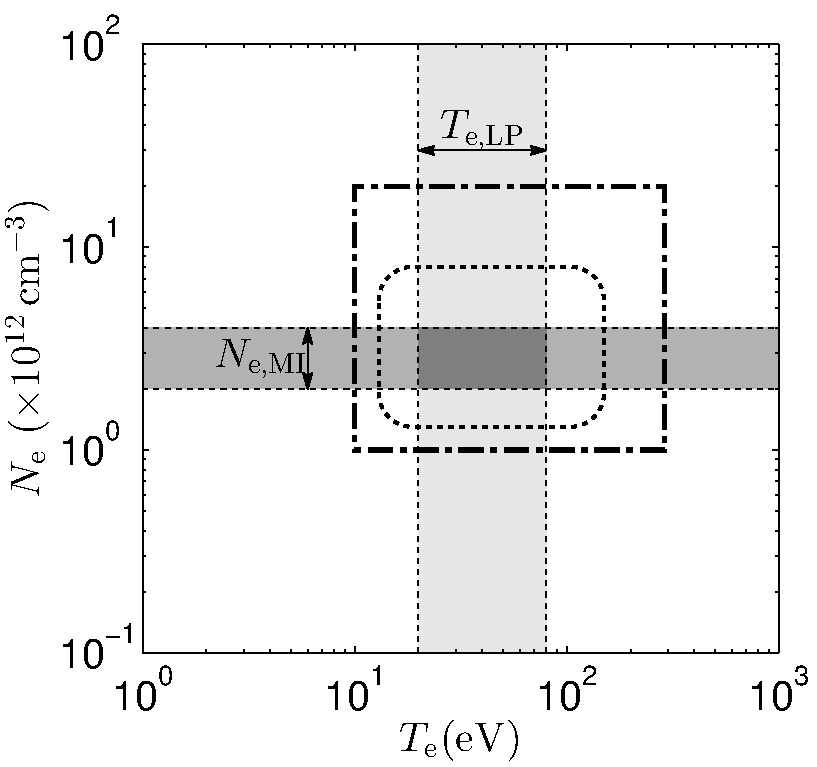
\includegraphics[width=\textwidth]{sunist_parram_vs_lineratio_range}
	\end{columns}
	\vspace{-1.2em}
	\begin{itemize}
		\item 在 SUNIST 上开展氦原子发射谱线诊断研究的意义
			\begin{itemize}
				\item 建立适用于小型托卡马克装置放电的碰撞辐射模型
					\begin{itemize}
						\item 研究包含不同的能级数时对计算结果的影响
						%验证在小型磁约束装置上的适用性
						\item 对速率系数精度要求给出直接的判断标准
						%\item 研究模型包含不同能级数、速率系数不确定性传递规则等
						%\item 研究激发态能级数预测误差对谱线比的影响
					\end{itemize}
				\item 为 SUNIST 建立起光谱诊断手段%基础
%					\begin{itemize}
%						\item 建立光谱诊断、微波诊断、数据采集等系统并改善放电重复性
%					\end{itemize}
%				\item 积累氦原子光谱诊断经验,希望能为国内其他装置提供参考
			\end{itemize}
	\end{itemize}
\end{frame}

\subsection{课题研究思路与内容}

\begin{frame}{课题研究思路与各部分内容的关系}
	\begin{itemize}
		\item 研究思路与内容\\
			\begin{center}
			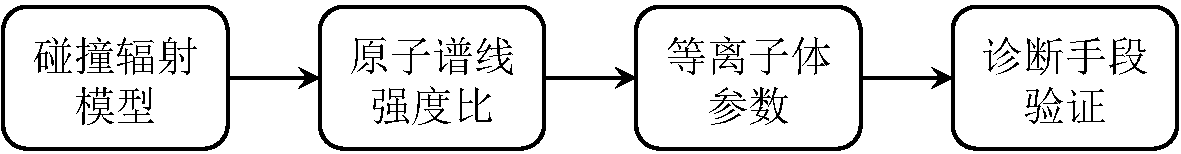
\includegraphics[width=0.7\textwidth]{research-progress}
			\end{center}
		\item 研究内容之间的详细关系\\
			\begin{center}
			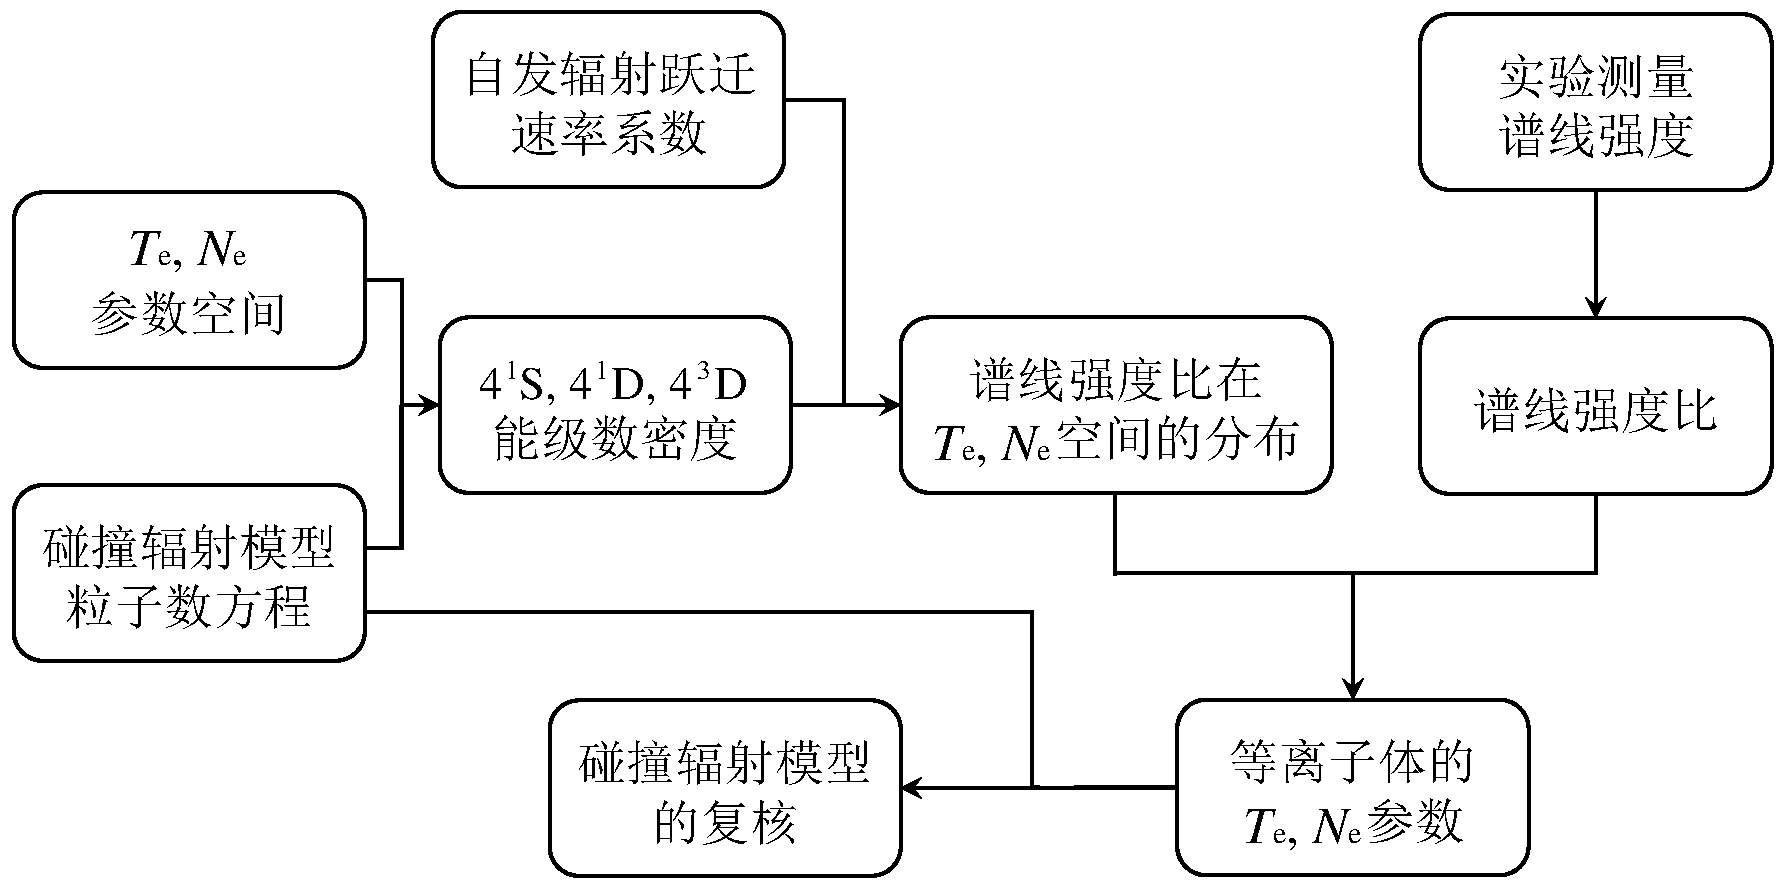
\includegraphics[width=0.8\textwidth]{lineratio-method-rellevelabun}
			\end{center}
	\end{itemize}
\end{frame}

\section{SUNIST 参数范围下氦原子的碰撞辐射模型与谱线比法}

\subsection{碰撞辐射模型的建立}

%\subsection{SUNIST 氦放电等离子体的特点}
%
%\begin{frame}{SUNIST 氦放电等离子体的主要粒子}
%	\begin{columns}
%	\column{0.5\textwidth}
%	\begin{itemize}
%		\item
%	\end{itemize}
%	\column{0.5\textwidth}
%	\end{columns}
%\end{frame}

\begin{frame}{氦放电等离子体激发态数密度分布特点与能级结构}
	\begin{columns}
		\column{0.45\textwidth}
			\begin{itemize}
				\item 临界能级主量子数\\ \onlineref{H.R. Griem (1964)}
					\[
					\hspace{-1em}
					n_c=\left(\frac{8\cdot10^{17}}{N_e}\right)^{2/17}
        			\left(\frac{kT_e}{\chi_H}\right)^{1/17}
        			\]
        		\item 氦激发态能级分布\\ \onlineref{Fujimoto JQSRT(1979)}
        			\begin{itemize}
						\item $N_p/g_p\propto n^{-0.5}\,(n<n_c)$
						\item $N_p/g_p\propto n^{-6}\,(n>n_c)$
					\end{itemize}
				\item SUNIST 等离子体
					\begin{itemize}
						\item 高温低密度:$n_c\simeq 6$
						\item 低温高密度:$n_c\simeq 4$
					\end{itemize}
			\end{itemize}
		\column{0.55\textwidth}
			\centering
			SUNIST 碰撞辐射模型~He~原子能级图\\[1em]
			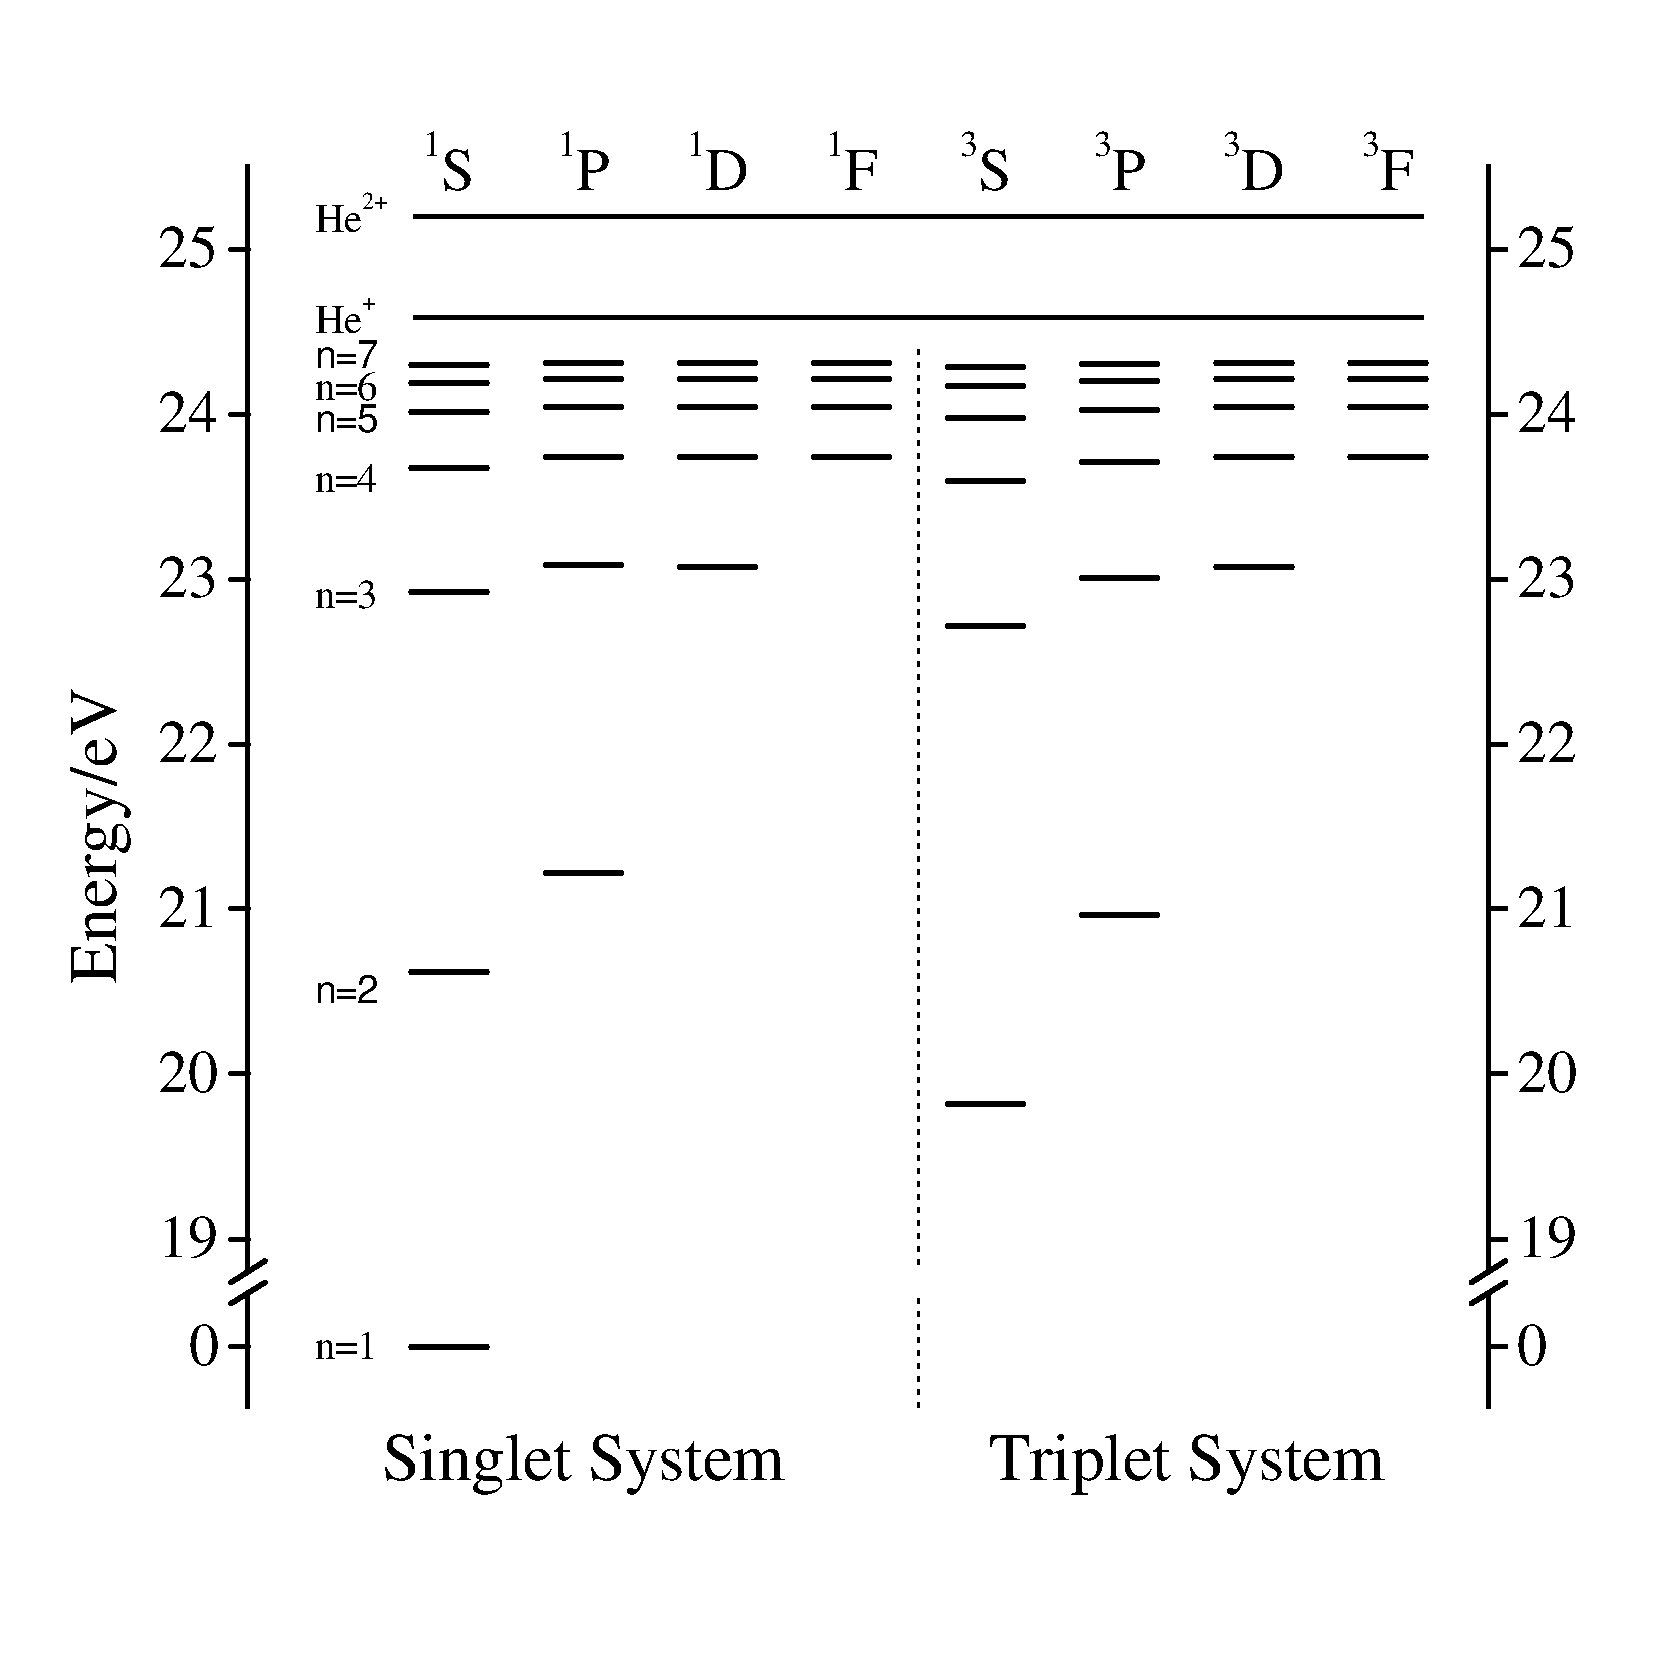
\includegraphics[width=\textwidth]{He-diagrames-plus-wlxb-en}
	\end{columns}
\end{frame}

\begin{frame}{电子碰撞与重粒子碰撞过程的反应速率}
	$$
	\frac{{\rm d}\,N_p}{{\rm d}\,t}=-n_{\rm e,X}\cdot N_p\cdot <v_{\rm e,X}\cdot\sigma_{pq}>
	$$
\end{frame}

\begin{frame}{电子碰撞与重粒子碰撞激发过程的选择}
\centering
%氦原子电子碰撞(${\rm e-}$)和重粒子碰撞(${\rm X-}$)激发过程的量级
\begin{table}%[H]
\begin{center}
%{\small 其中,${\rm exc}$ 表示激发过程,${\rm ion}$ 表示电离过程,${\rm dbion}$ 表示双电子离过程}\\
\begin{tabular}{lrrrrc}\toprule[1.5pt]
反应过程 & $n_{\rm e,X}$ & $N_{p}$ & $v_{\rm e,X}$ & $\sigma_{pq}$ & 反应过程量级\\
\midrule[1pt]
${\rm e-}$基态       & $+6$ & $0$  & $0$  & $0$  & $+6$ \\
${\rm e-}$亚稳态     & $+6$ & $-1$ & $0$  & $0$  & $+5$ \\
${\rm e-}$普通激发态 & $+6$ & $-4$ & $0$  & $0$  & $+2$ \\
\color{gray}{${\rm X-}$基态} & \color{gray}{$+4$} & \color{gray}{$0$}  & \color{gray}{$-3$} & \color{gray}{$-3$} & \color{gray}{$-2$} \\
\color{gray}{${\rm X-}$亚稳态}     & \color{gray}{$+4$} & \color{gray}{$-1$} & \color{gray}{$-3$} & \color{gray}{$-3$} & \color{gray}{$-3$} \\
\color{gray}{${\rm X-}$普通激发态} & \color{gray}{$+4$} & \color{gray}{$-4$} & \color{gray}{$-3$} & \color{gray}{$-3$} & \color{gray}{$-6$} \\
\bottomrule[1.5pt]
\end{tabular}
\end{center}
\end{table}
\end{frame}

\begin{frame}{电子碰撞与重粒子碰撞电离过程的选择}
\centering
%氦原子电子碰撞(${\rm e-}$)和重粒子碰撞(${\rm X-}$)电离过程的量级
\begin{table}%[H]
\begin{center}
%{\small 其中,${\rm exc}$ 表示激发过程,${\rm ion}$ 表示电离过程,${\rm dbion}$ 表示双电子离过程}\\
\begin{tabular}{lrrrrc}\toprule[1.5pt]
反应过程 & $n_{\rm e,X}$ & $N_{p}$ & $v_{\rm e,X}$ & $\sigma_{pq}$ & 反应过程量级\\
\midrule[1pt]
${\rm e-}$基态       & $+6$ & $0$  & $0$  & $+1$ & $+7$ \\
${\rm e-}$亚稳态     & $+6$ & $-1$ & $0$  & $+1$ & $+6$ \\
${\rm e-}$普通激发态 & $+6$ & $-4$ & $0$  & $+1$ & $+3$ \\
\color{gray}{${\rm X-}$基态}       & \color{gray}{$+4$} & \color{gray}{$0$}  & \color{gray}{$-3$} & \color{gray}{$-3$} & \color{gray}{$-2$} \\
\color{gray}{${\rm X-}$亚稳态}     & \color{gray}{$+4$} & \color{gray}{$-1$} & \color{gray}{$-3$} & \color{gray}{$-3$} & \color{gray}{$-3$} \\
\color{gray}{${\rm X-}$普通激发态} & \color{gray}{$+4$} & \color{gray}{$-4$} & \color{gray}{$-3$} & \color{gray}{$-3$} & \color{gray}{$-6$} \\
${\rm e-}$基态(双电离)       & $+6$ & $0$  & $0$  & $-2$  & $+4$ \\
\color{gray}{${\rm e-}$亚稳态(双电离)}     & \color{gray}{$+6$} & \color{gray}{$-1$} & \color{gray}{$0$}  & \color{gray}{$-2$}  & \color{gray}{$+3$} \\
\color{gray}{${\rm e-}$普通激发态(双电离)} & \color{gray}{$+6$} & \color{gray}{$-4$} & \color{gray}{$0$}  & \color{gray}{$-2$}  & \hspace{0.8em}\color{gray}{$0$} \\
\color{gray}{${\rm X-}$基态(双电离)}       & \color{gray}{$+4$} & \color{gray}{$0$}  & \color{gray}{$-3$} & \color{gray}{$-3$} & \color{gray}{$-2$} \\
\color{gray}{${\rm X-}$亚稳态(双电离)}     & \color{gray}{$+4$} & \color{gray}{$-1$} & \color{gray}{$-3$} & \color{gray}{$-3$} & \color{gray}{$-3$} \\
\color{gray}{${\rm X-}$普通激发态(双电离)} & \color{gray}{$+4$} & \color{gray}{$-4$} & \color{gray}{$-3$} & \color{gray}{$-3$} & \color{gray}{$-6$} \\
\bottomrule[1.5pt]
\end{tabular}
\end{center}
\end{table}
\end{frame}


\begin{frame}{速率方程:基态}
	\[
	\begin{aligned}
		\frac{{\rm d}\,N_1}{{\rm d}\,t}=
			&-\left\{\sum_{q>1}C_{1q}+S_{{\rm He}^+}(1)+S_{{\rm He}^{2+}}(1)\right\}N_{\rm e}N_1\\
			&+\sum_{q>1}\left\{C_{q1}N_{\rm e}+A_{q1}\right\}N_q\\
			&+\left\{\beta_{{\rm He}^+}(1)+\beta_{{\rm He}^+,\rm d}(1)\right\}N_{\rm e}N_{{\rm He}^+}
	\end{aligned}
	\]
	\begin{itemize}
		\item 主要损失过程:电子碰撞激发与电离
		\item 主要产生过程:电子碰撞退激发、激发态自发辐射跃迁、
			${\rm He}^+$ 离子的辐射复合 (radiation recombination)
			与双电子复合 (dielectric recombination)
	\end{itemize}
\end{frame}

\begin{frame}{速率方程:亚稳态~($2^1{\rm S}$~和~$2^3{\rm S}$)~与普通激发态}
	\[
	\begin{aligned}
		\frac{{\rm d}\,N_p}{{\rm d}\,t}=
		&-\left\{\sum_{q\ne p}C_{pq}N_{\rm e}+\sum_{q<p}A_{pq}+S_{{\rm He}^+}(p)N_{\rm e}\right\}N_p\\
		&+\left\{\sum_{q\ne p}C_{qp}N_{\rm e}+\sum_{q>p}A_{qp}\right\}N_q\\
		&+\beta_{{\rm He}^+}(p)N_{\rm e}N_{{\rm He}^+}
	\end{aligned}
	\]
	\begin{itemize}
		%\item 忽略过程:电子碰撞双电子电离与双电子复合
		\item 主要损失过程:电子碰撞激发/退激发、电离与自发辐射跃迁
		\item 主要产生过程:电子碰撞激发/退激发、${\rm He}^+$ 辐射复合与自发辐射跃迁
	\end{itemize}
\end{frame}

\begin{frame}{速率方程:${\rm He}^+$ 离子}
	\[
	\begin{aligned}
		\frac{{\rm d}\,N_{{\rm He}^+}}{{\rm d}\,t}=
		&-\left\{\sum_{p}\beta_{{\rm He}^+}(p)+\beta_{{\rm He}^+,{\rm d}}(1)+S_{{\rm He}^{2+}}({\rm He}^+)\right\}N_{\rm e}N_{{\rm He}^+}\\
		&+N_{\rm e}\sum_{p}S_{{\rm He}^+}(p)N_p+\beta_{{\rm He}^{2+}}({\rm He}^{+})N_{\rm e}N_{{\rm He}^{2+}}
	\end{aligned}
	\]
	\begin{itemize}
		\item 主要损失过程:电子碰撞电离、辐射复合与双电子复合过程
		\item 主要产生过程:激发态碰撞电离、${\rm He}^{2+}$ 复合
	\end{itemize}
\end{frame}

\begin{frame}{速率方程:${\rm He}^{2+}$ 离子}
	\[
	\begin{aligned}
		\frac{{\rm d}\,N_{{\rm He}^{2+}}}{{\rm d}\,t}=
			&-\beta_{{\rm He}^{2+}}({\rm He}^{+})N_{\rm e}n_{{\rm He}^{2+}}\\
			&+\left\{S_{{\rm He}^{2+}}(1)N_1+S_{{\rm He}^{2+}}({\rm He}^+)N_{{\rm He}^+}\right\}N_{\rm e}
	\end{aligned}
	\]
	\begin{itemize}
		\item 主要损失过程:电子碰撞复合至 ${\rm He}^+$ 离子
		\item 主要产生过程:基态原子与 ${\rm He}^+$ 离子的电子碰撞电离
	\end{itemize}
\end{frame}



\begin{frame}{准稳态近似处理}
	对~SUNIST~中等离子体的各时间常数分析\onlineref{H.P. Summers PPCF(2006)}:
	\begin{description}
		\item[原子内在固有时间常数:辐射、跃迁相关]
			\quad\\
			\hspace{-3em}
			$\tau_{\rm rad-ion}\sim 10^{-13}{\rm s}\,{\color{red} <}\,
			\tau_{\rm ord-rad}\sim \frac{10^{-8}}{z^4}{\rm s}\,{\color{red} <}\,
			\tau_{\rm meta-rad}\sim \frac{10^{1}}{z^8}{\rm s}$
		\item[外在时间常数:受 $T_{\rm e}$、$N_{\rm e}$ 影响]
			\quad\\
			\hspace{-3em}
			$\tau_{\rm e-e}\sim 4 {\rm \mu s}\,{\color{red} <}\,
            \tau_{\rm i-i}\sim 20 {\rm \mu s}\,{\color{red} <}\,
            \tau_{\rm e-ion}\sim 1.4 {\rm \mu s} - 140 {\rm \mu s}\,{\color{red} <}\,
            \tau_{\rm i-e}\sim 2 {\rm ms}$
		\item[与等离子体行为相关时间参数~$\tau_{\rm{plasma}}$~对比]
			\quad\\
			\hspace{-3em}
			${\color{magenta}\tau_{\rm ord-rad}} \,{\color{red} <}\,
            \tau_{\rm e-e,i-i} \,{\color{red} <}\,
            {\color{magenta}\tau_{\rm e-ion}} \,{\color{red} <}\,
            \tau_{\rm plasma}$%\sim\tau_{gs}\sim\tau_{m}$

			$\tau_{\rm{plasma}}$:等离子体在空间尺度上扩散、输运等时间常数
			%$\tau_{\rm{plasma}}$~表示粒子在 $T_{\rm e}$、$N_{\rm e}$ 梯度尺度范围扩散、输运等过程时间常数
	\end{description}
	
	\begin{itemize}%[<2->]
		\item 准稳态近似处理:%的一些优点:
			\begin{itemize}
				\item 局域计算中, 不考虑粒子扩散输运等过程
				\item 联立速率方程,求其稳态解
				%\item 粒子数方程中只存是基态, 亚稳态, 以及离子等
				%\item 普通激发态粒子数平衡方程退化为线性耦合方程
				\item 放电平顶段适用
			\end{itemize}
%		\item H. Griem提出能级高于主量子数为$n_c^p$的能级处于准饱和区
%			\myfootnote{Plasma Spectroscopy, p. 129, McGraw-Hill, New York(1964)}
%			,其反应过程为阶梯型,且粒子数密度随能级升高急剧下降
%		\item 对于SUNIST等离子体,高密度下$n_c^p=4$,低密度下$n_c^p=6$
	\end{itemize}

\end{frame}

\begin{frame}{等效电荷数计算结果与 FLYCHK 对比}
	\centering
	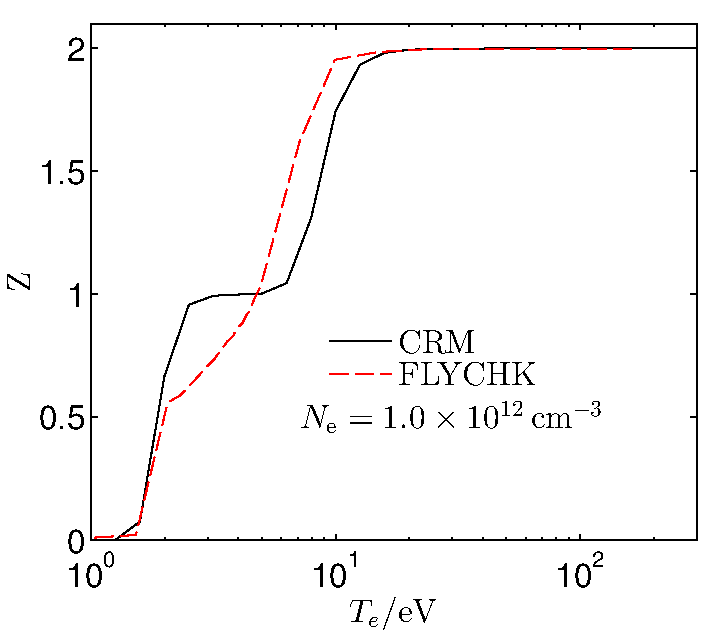
\includegraphics[width=0.6\textwidth]{ZvsTe-spec-Ne-1_0E2}
\end{frame}

\subsection{碰撞辐射模型的研究}

\begin{frame}{速率系数不确定性:各能级的主要产生过程}
	\centering
	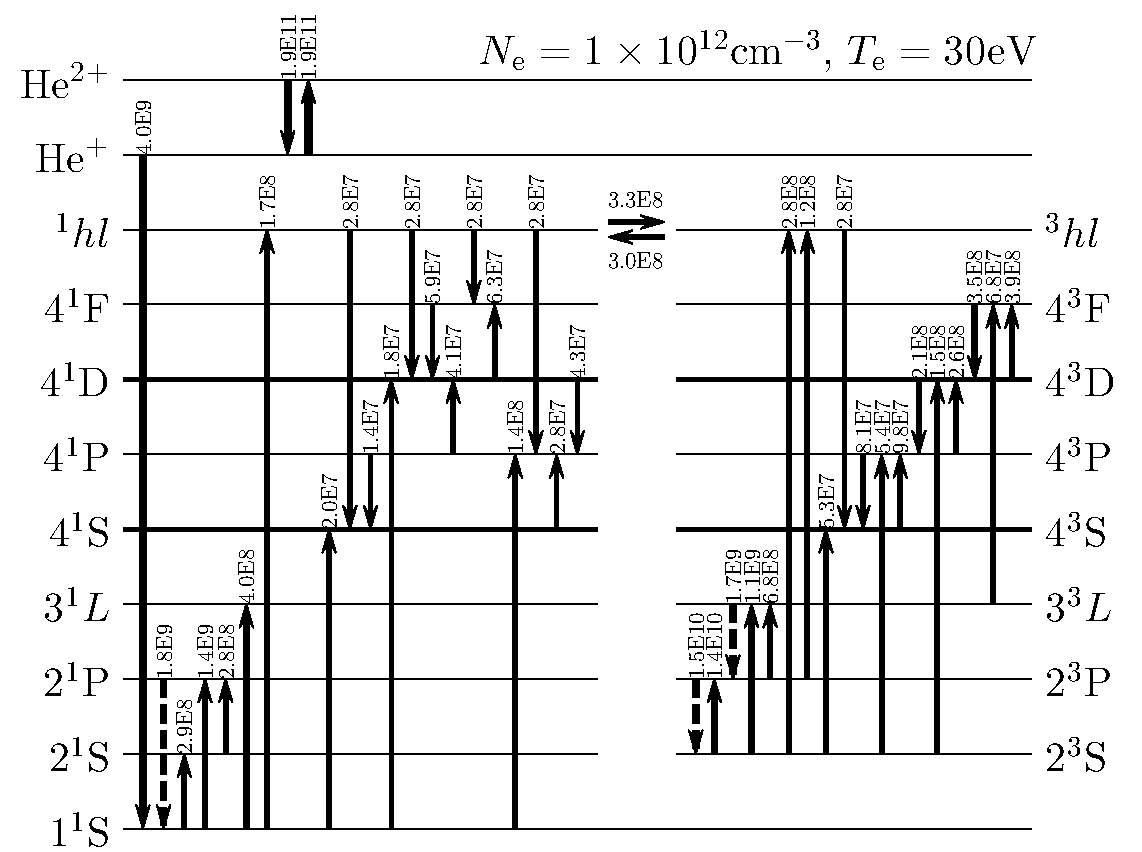
\includegraphics[height=0.8\textheight]{Ne1E12_Te30_1e7cm-3s-1}
\end{frame}

\begin{frame}{速率系数不确定性:速率系数不确定性传递函数}
	\centering
	对于普通激发态能级,电子碰撞电离与复合过程均不超过 $10\%$
	$$\Longrightarrow N_{\rm e}\sum_{i\ne p}C_{ip}N_i=N_{\rm e}N_p\sum_{i\ne p}C_{pi}+N_p\sum_{i<p}A_{pi}$$
	$$\Longrightarrow \sigma_{N_p}=\frac{{\rm d}N_p}{N_p} = \sigma\left(N_{\rm e}\sum_{i\ne p}C_{ip}N_i\right) + \sigma\left(N_{\rm e}\sum_{i\ne p}C_{pi}+\sum_{i<p}A_{pi}\right)$$
	$$\Longrightarrow \sigma_{N_p}=\alert{E_{jp}}\sigma_{C_{jp}}\simeq\alert{2\frac{f_{jp}}{F_{p,{\rm in}}}}\sigma_{C_{jp}}$$
	\begin{itemize}
		\item $E_{jp}$ 的物理意义
			\begin{itemize}
				\item 该过程占能级总产生速率的比例越重,其速率系数不确定性至激发态粒子数密度计算结果的传递越明显
				\item 其逆过程的粒子流速率相应变化,则会出现 2 倍的系数
				\item 据此,可以\alert{直接}对速率系数准确性提出具体要求
			\end{itemize}
	\end{itemize}
\end{frame}

\begin{frame}{速率系数不确定性:不确定性传递计算结果}
	%\vspace{-0.5em}
	\begin{columns}
	\column{0.65\textwidth}
	\begin{itemize}
        %\item the uncertainties of the rates between the same $n$ and those from $hl$ dominate the error in population densities of the excited states
		%\item Based on the analysis of $n=3$ states
%        \item 单一速率系数具不确定性
%        \item[] $\Rightarrow$
%        \item 最大相对误差:$\sigma_{N_p}=E_{jp}\sigma_{C_{jp}}\simeq2\frac{f_{jp}}{F_{p,in}}\sigma_{C_{jp}}$
		\item 对相同主量子数的相邻能级、基态和高能级的总和的速率系数要求高
		\item 相邻能级速率系数单一变化时,对模型计算结果影响可达 $40\%$
	\end{itemize}
	\column{0.3\textwidth}
\begin{small}
\begin{tabular}{lc}
\toprule
跃迁类型 & 误差\\
\hline
基态$\to$单重态  & $\pm10\%$ \\
基态$\to$三重态  & $\pm15\%$ \\
亚稳态$\to$其他  & $\pm20\%$ \\
其他过程  & $\pm50\%$ \\
\bottomrule
\end{tabular}
\end{small}
	%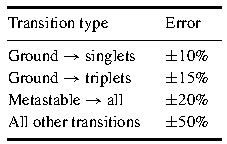
\includegraphics[width=\textwidth]{exc_rates_error_cropped}
	\end{columns}
	\vspace{1em}
	\begin{columns}
			\column{0.45\textwidth}
				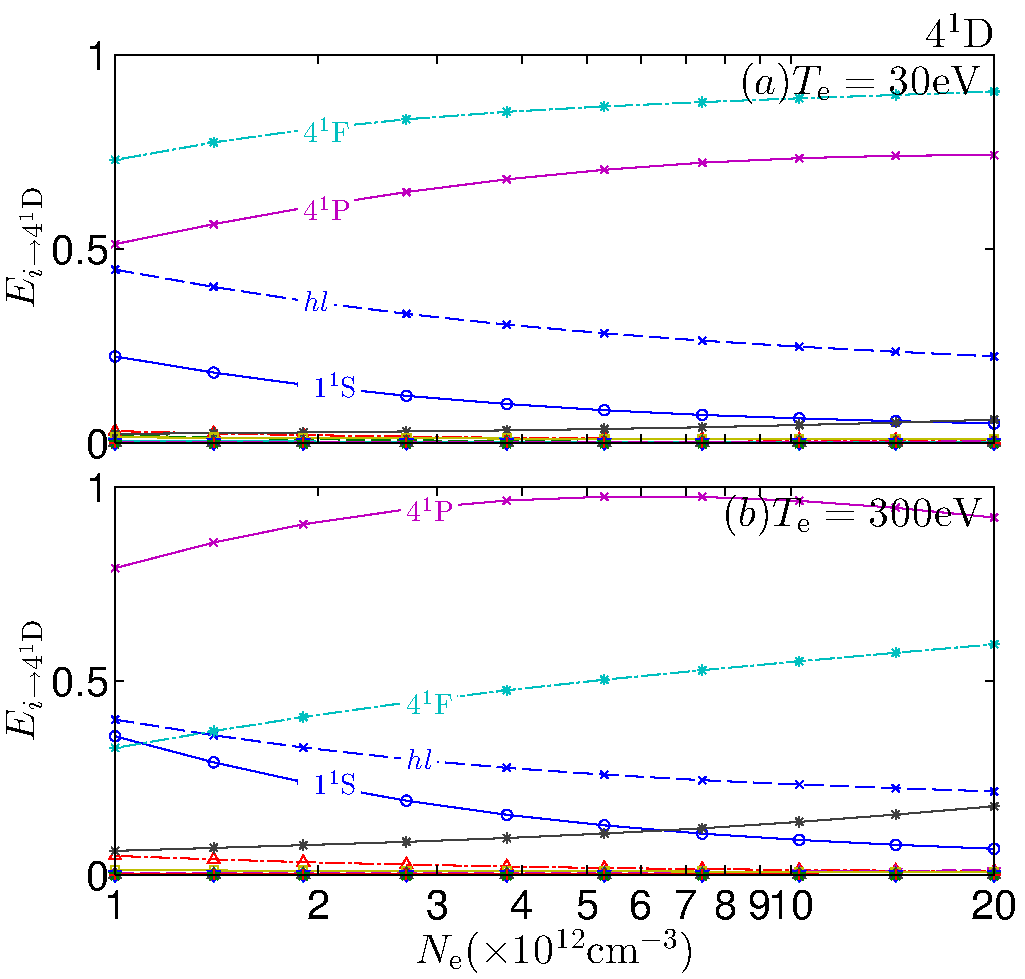
\includegraphics[width=\textwidth]{41D-error-propagation-coefficient}\\
				%\mbox{\tiny [\texttt{N. Brenning J.Phys.D (1980)}]}
			\column{0.04\textwidth}
				$\Longrightarrow$
%			\column{0.2\textwidth}
%				\vspace{2.5cm}
%				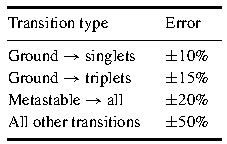
\includegraphics[width=\textwidth]{exc_rates_error_cropped}\\
%				\vspace{2.1cm}
%				%\mbox{{\tiny [\texttt{Y Andrew PPCF(2000)}]}$\to$}
%			\column{0.02\textwidth}
%				$\Rightarrow$
			\column{0.45\textwidth}
				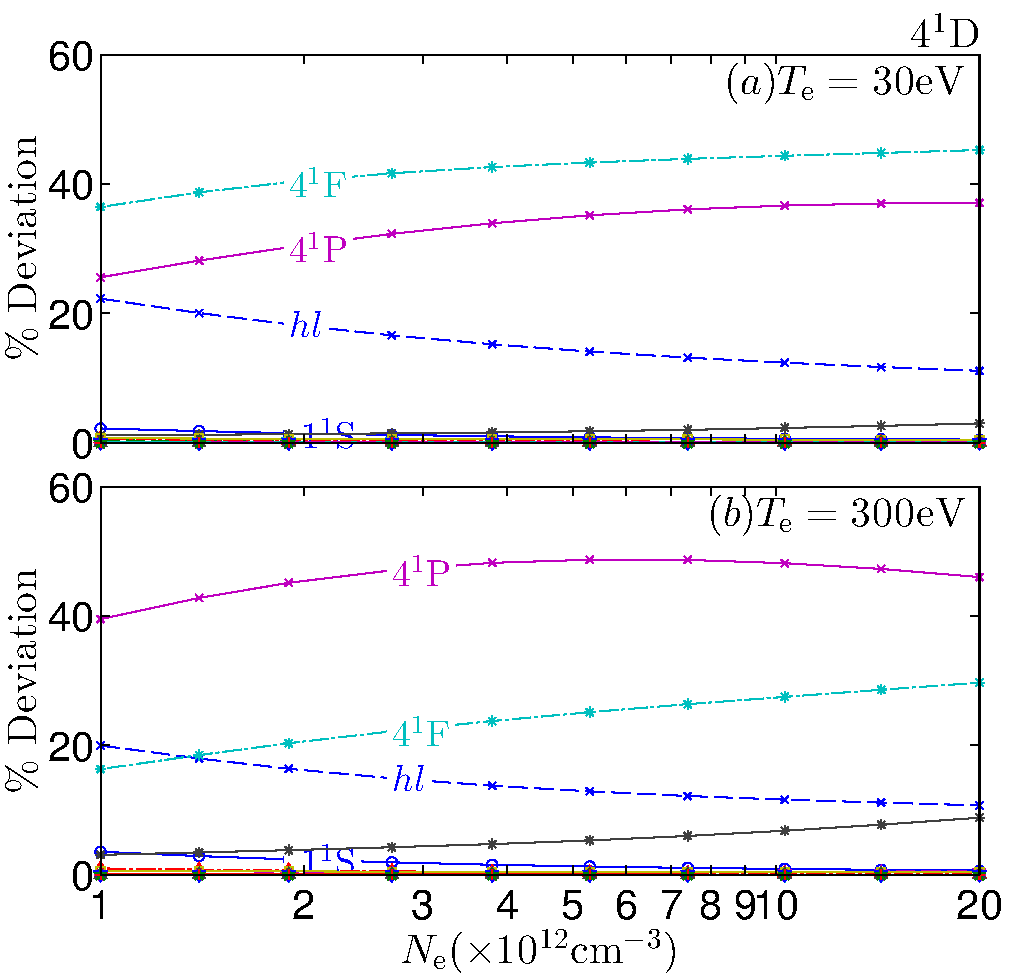
\includegraphics[width=\textwidth]{41D-error-propagation}
	\end{columns}
\end{frame}


\begin{frame}{模型中包含的能级对激发态数密度计算结果的影响}%
		\begin{columns}[T]
	\column{0.6\textwidth}
	\vspace{-0.7cm}
	\begin{center}
		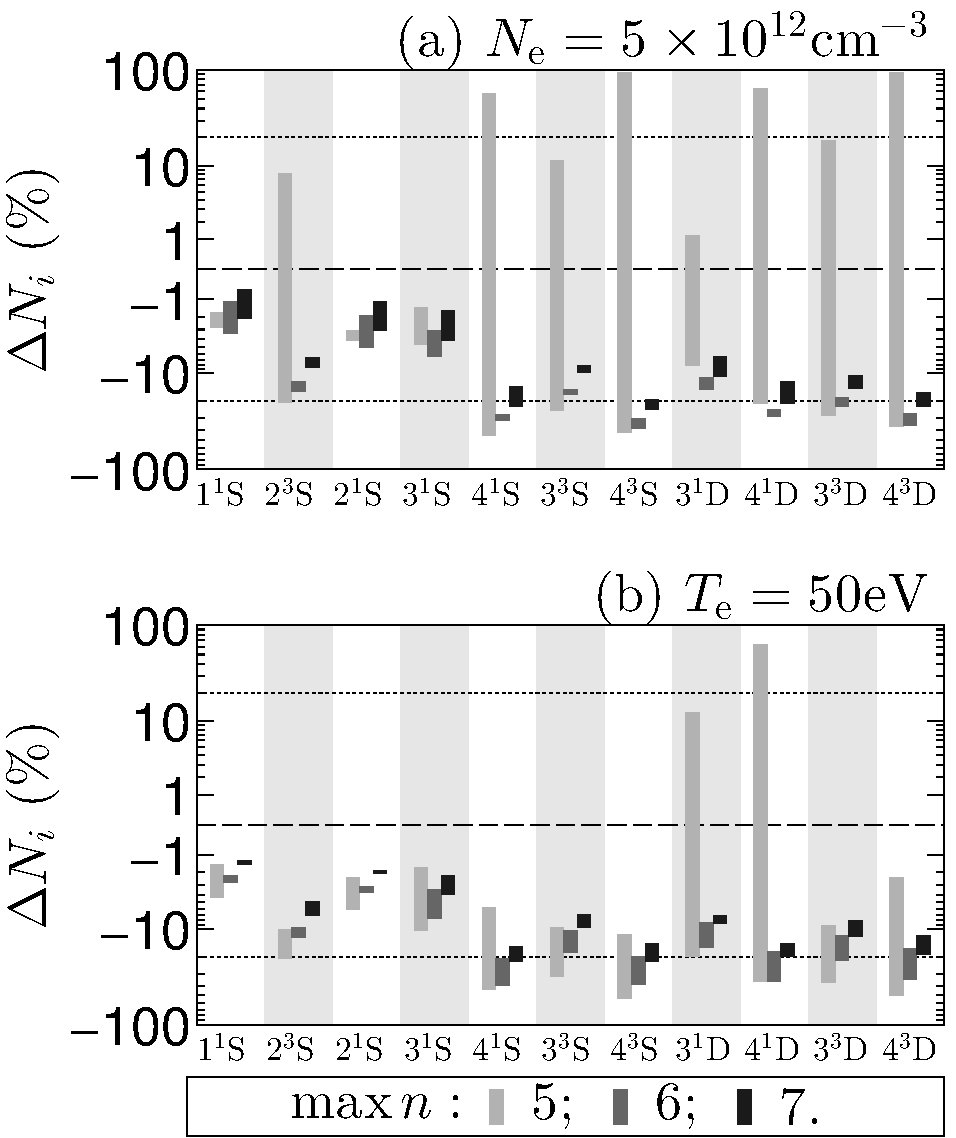
\includegraphics[height=0.9\textheight]{levelabun-reldiff-maxn5to7-allstates}
	\end{center}
	
	\column{0.3\textwidth}
	\begin{align*}
	   \Delta N_i^{\max n} & = 100\% \times \\
    	 & \frac{N_i^{\max n}-N_i^{\max n-1}}{N_i^{\max n-1}}
	\end{align*}
    \vspace{1em}
    %\pause
%    \begin{itemize}
%        \item 对谱线比计算结果的影响:
%    \end{itemize}
%    \begin{align*}
%    \sigma_{r^{\rm mod}} & \simeq\pm r^{\rm mod}\times \\
%    & \sqrt{2\left(\frac{\sigma_n}{n}\right)^2(1-\gamma_{qj})}
%    \end{align*}
%    \onlineref{Burgos PoP (2012)}
	\end{columns}
\end{frame}

%\begin{frame}{对谱线比计算结果的影响}
%	\begin{itemize}
%        \item 对谱线比计算结果的影响\onlineref{Burgos PoP (2012)}:
%    \end{itemize}
%    \begin{align*}
%    \sigma_{r^{\rm mod}} & \simeq\pm r^{\rm mod}\times \\
%    & \sqrt{2\left(\frac{\delta n}{n}\right)^2(1-\gamma_{qj})}
%    \end{align*}
%
%\end{frame}

%\begin{frame}{能级计算误差对谱线比计算结果的影响}
%\end{frame}
\subsection{诊断 $T_{\rm e}$ 和 $N_{\rm e}$ 谱线比法的建立}

\begin{frame}{谱线比选择}
	\begin{center}{\tiny
		\begin{tabular}{ccc}\toprule
			跃迁 & \makecell[c]{$\lambda_{q\to p}$\\ (${\rm nm})$} & \makecell[c]{$A_{q\to p}^{\rm eff}$\\ ($10^7\,{\rm s}^{-1}$)}\\
			\hline
			{\color{red}$2^1{\rm S}\leftarrow3^1{\rm P}$} & {\color{red}501.6} & {\color{red}1.34} \\
			{\color{red}$2^1{\rm S}\leftarrow4^1{\rm P}$} & {\color{red}396.5} & {\color{red}0.70} \\
			$2^1{\rm P}\leftarrow4^1{\rm S}$ & 504.8 & 0.68 \\
			$2^1{\rm P}\leftarrow4^1{\rm D}$ & 492.2 & 1.99 \\
			{\color{red}$2^3{\rm S}\leftarrow3^3{\rm P}$} & {\color{red}388.9} & {\color{red}0.95} \\
			$2^3{\rm P}\leftarrow3^3{\rm D}$ & 587.6 & 7.07 \\
			$2^3{\rm P}\leftarrow4^3{\rm S}$ & 471.3 & 0.95 \\
			$2^3{\rm P}\leftarrow4^3{\rm D}$ & 447.1 & 2.46 \\
			{\color{magenta}$2^3{\rm P}\leftarrow5^3{\rm S}$} & {\color{magenta}412.1} & {\color{magenta}0.45} \\
			\bottomrule
		\end{tabular}
		}\\
		{\color{green}\fbox{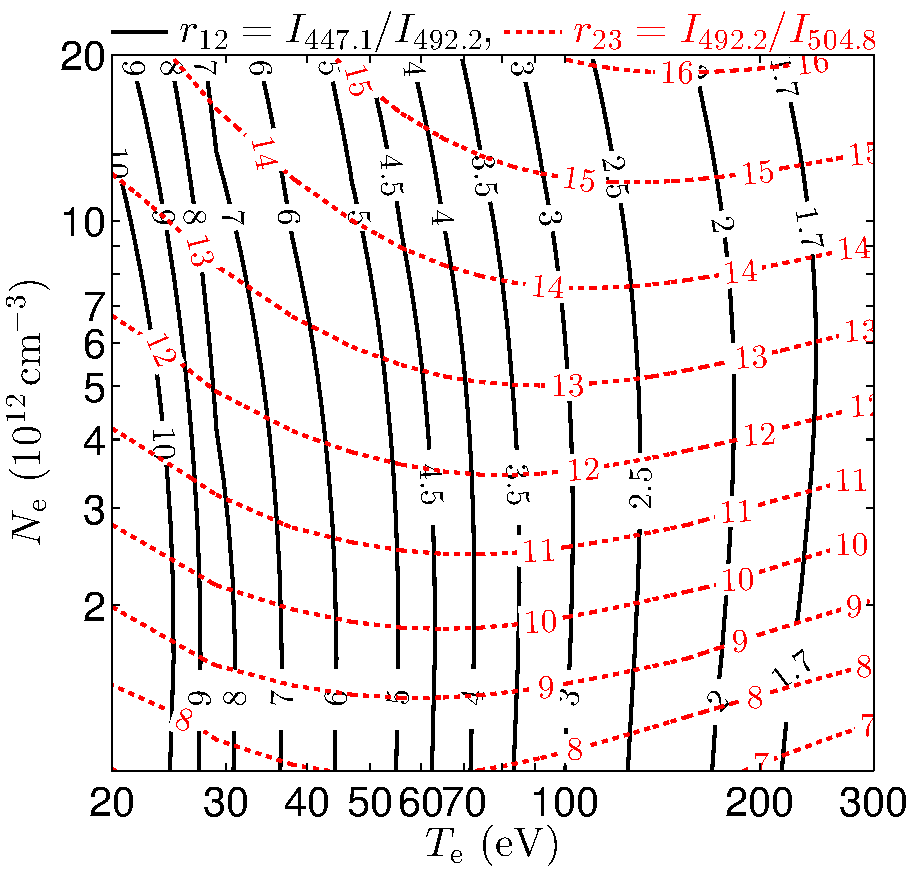
\includegraphics[width=0.32\textwidth]{1-9to7-7to5-getTeNe-lineratio}}}
		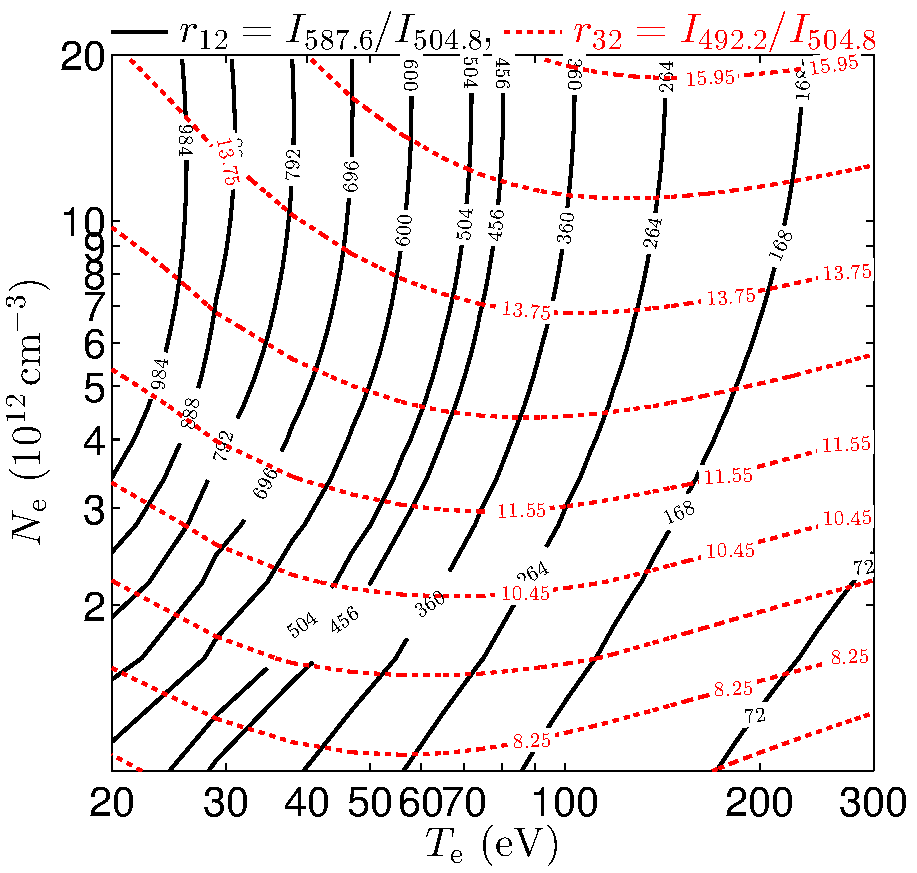
\includegraphics[width=0.32\textwidth]{1-4to5-7to5-getTeNe-lineratio}
		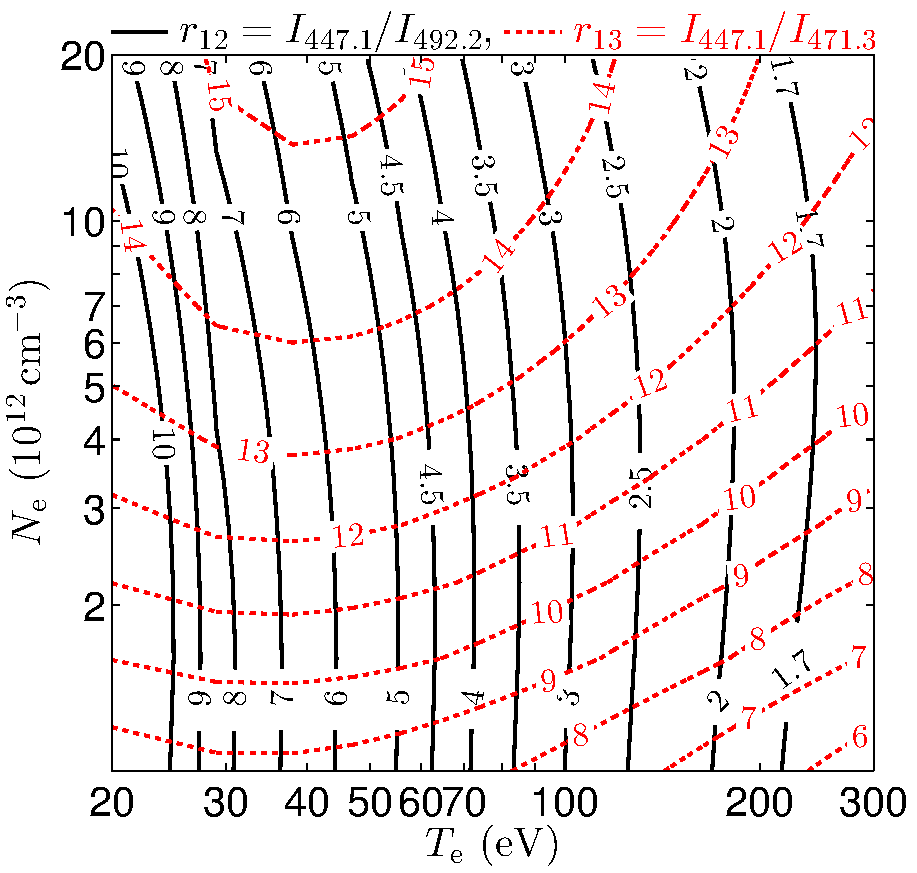
\includegraphics[width=0.32\textwidth]{1-9to8-9to7-getTeNe-lineratio}
	\end{center}
\end{frame}

\begin{frame}{碰撞辐射模型对谱线比的预测}
	\vspace{-0.3cm}
	\begin{center}
		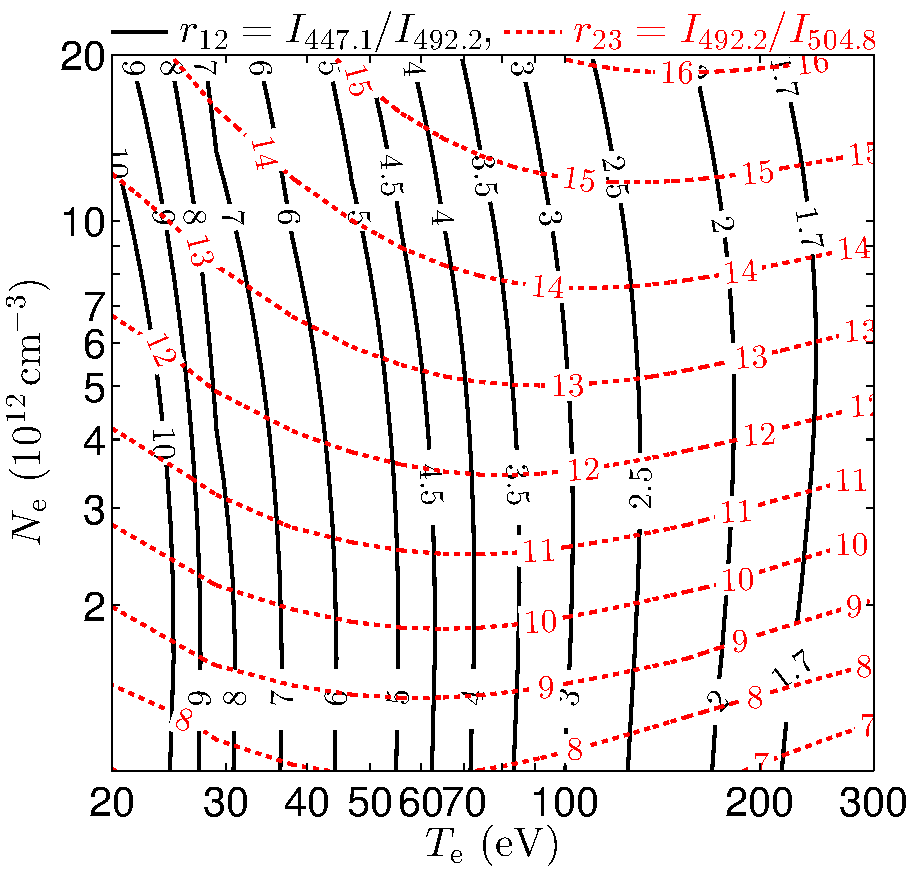
\includegraphics[height=0.9\textheight]{1-9to7-7to5-getTeNe-lineratio}
	\end{center}
\end{frame}

\begin{frame}{谱线比法确定 $T_{\rm e}$ 和 $N_{\rm e}$}
	\vspace{-0.3cm}
	\begin{center}
		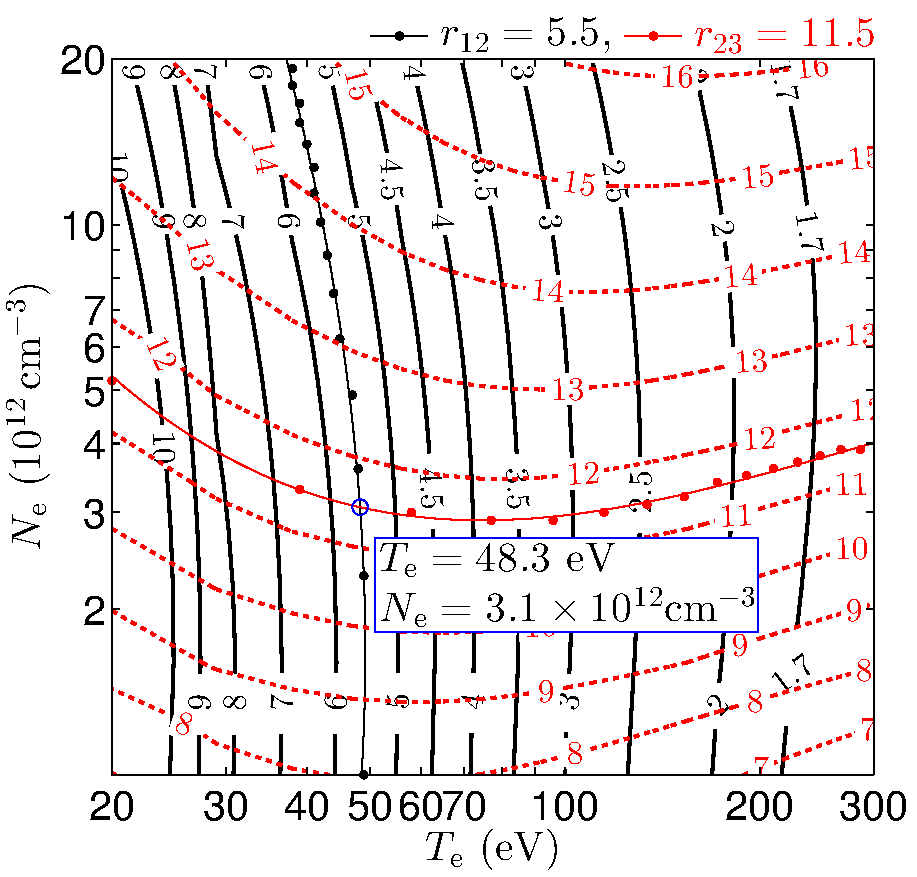
\includegraphics[height=0.9\textheight]{5-9to7-7to5-getTeNe-crosspoint}
	\end{center}
\end{frame}




\section{SUNIST 氦放电等离子体 $T_{\rm e}$ 与 $N_{\rm e}$ 的发射光谱诊断}

\subsection{SUNIST 原子发射光谱诊断实验测量系统与安排}

%\subsection{光谱诊断实验安排}

\begin{frame}{主要光谱测量设备}
	\begin{itemize}
		\item 两台单色仪:对两条谱线进行同时测量
			\begin{itemize}
				\item 可用谱线范围:380 nm -- 650 nm
				\item 焦距:1 m;光栅:2400 g/mm@400 nm;波长分辨率:0.004 nm;
				\\色散:0.4 nm/mm
				\item 光电倍增管:单点,但响应强,满足时间分辨测量要求
			\end{itemize}
		\bigskip
		\item 标定
			\begin{itemize}
				\item 汞灯:谱线准确度、分辨率
				\item 钨灯:仪器的整体响应
			\end{itemize}
		\bigskip
		\item 信号
			\begin{itemize}
				\item 取样电阻优化
				\item 屏蔽以降低噪声
				\item PMT 电源改造,消除来自电源干扰
			\end{itemize}
	\end{itemize}
\end{frame}

\begin{frame}{光谱测量安排}
	%\vspace{-0.3cm}
	\begin{columns}
	\column{0.5\textwidth}
	\begin{center}
		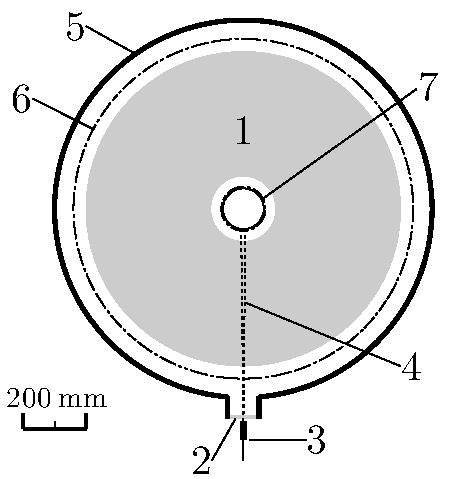
\includegraphics[height=0.6\textheight]{instru-alignments-2}
	\end{center}
	\column{0.5\textwidth}
\begin{tabular}{ccc}\toprule
跃迁 & \makecell[c]{$\lambda_{q\to p}$\\ (${\rm nm})$} & \makecell[c]{$A_{q\to p}^{\rm eff}$\\ ($10^7\,{\rm s}^{-1}$)}\\
\hline
$2^1{\rm S}\leftarrow3^1{\rm P}$ & 501.6 & 1.34 \\
$2^1{\rm S}\leftarrow4^1{\rm P}$ & 396.5 & 0.70 \\
$2^1{\rm P}\leftarrow4^1{\rm S}$ & 504.8 & 0.68 \\
$2^1{\rm P}\leftarrow4^1{\rm D}$ & 492.2 & 1.99 \\
$2^3{\rm S}\leftarrow3^3{\rm P}$ & 388.9 & 0.95 \\
$2^3{\rm P}\leftarrow3^3{\rm D}$ & 587.6 & 7.07 \\
$2^3{\rm P}\leftarrow4^3{\rm S}$ & 471.3 & 0.95 \\
$2^3{\rm P}\leftarrow4^3{\rm D}$ & 447.1 & 2.46 \\
$2^3{\rm P}\leftarrow5^3{\rm S}$ & 412.1 & 0.45 \\
\bottomrule
\end{tabular}
	\end{columns}
\end{frame}

\subsection{氦原子发射光谱测量结果}

\begin{frame}{氦放电等离子体电流与可见光信号}
	\centering
  \begin{figure}
      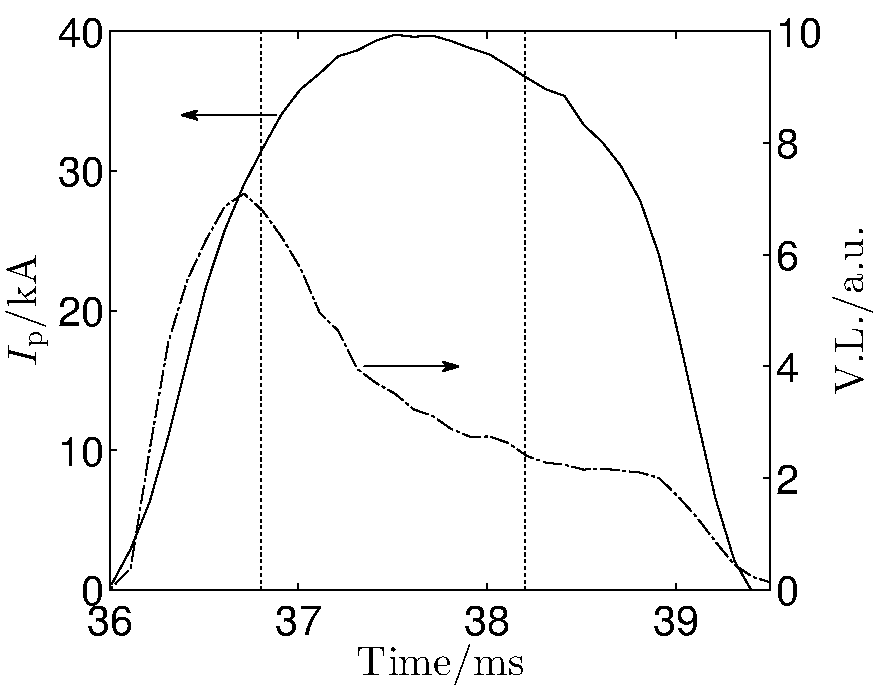
\includegraphics[height=0.6\textheight]{he-ip-and-vlight-for-gpxygpfx}
  \end{figure}
\end{frame}

\begin{frame}{谱线测量方法}
	\centering
  \begin{figure}
      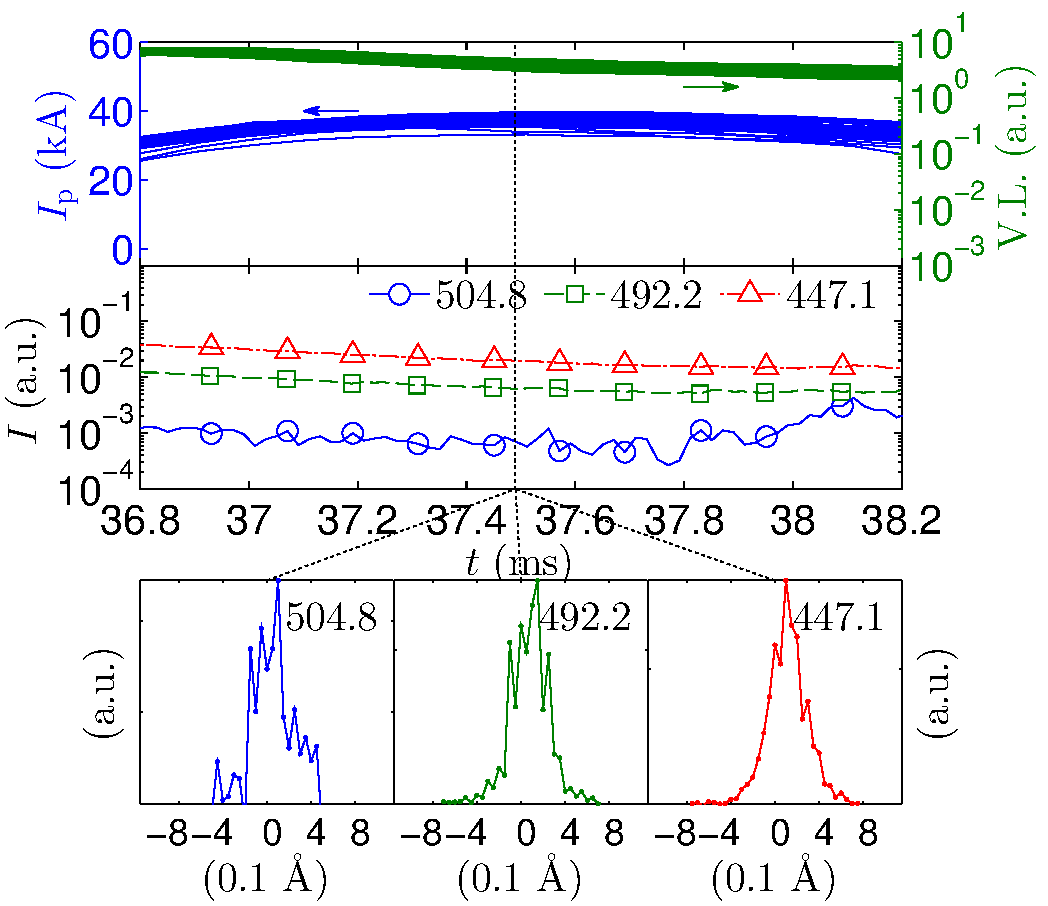
\includegraphics[height=0.8\textheight]{he-lines-shape-intensity-10-8-6-for-thesis}
  \end{figure}
\end{frame}

\begin{frame}{谱线测量结果}
	\centering
  \begin{figure}
      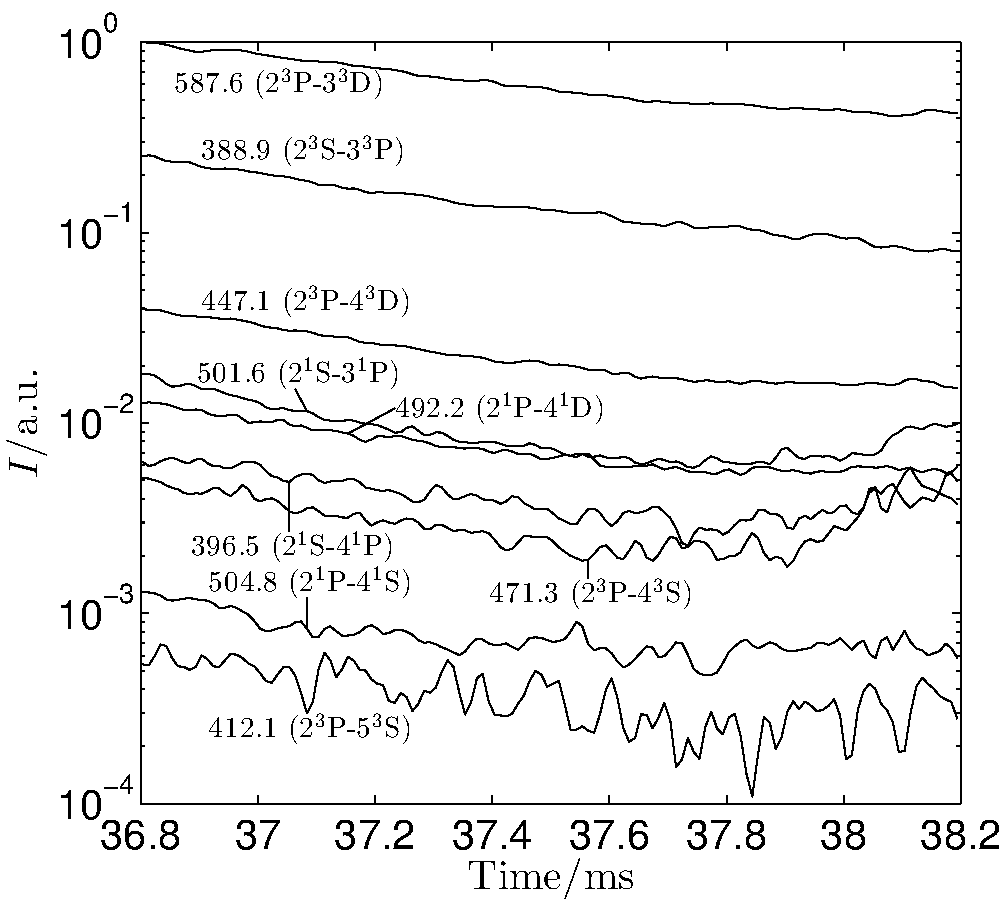
\includegraphics[height=0.8\textheight]{he-lines-whole-intensity-calibrated}
  \end{figure}
\end{frame}

\subsection{谱线比法诊断 $T_{\rm e}$ 和 $N_{\rm e}$}

\begin{frame}{谱线比法确定 $T_{\rm e}$ 和 $N_{\rm e}$}
	\vspace{-0.5em}
	\begin{figure}
      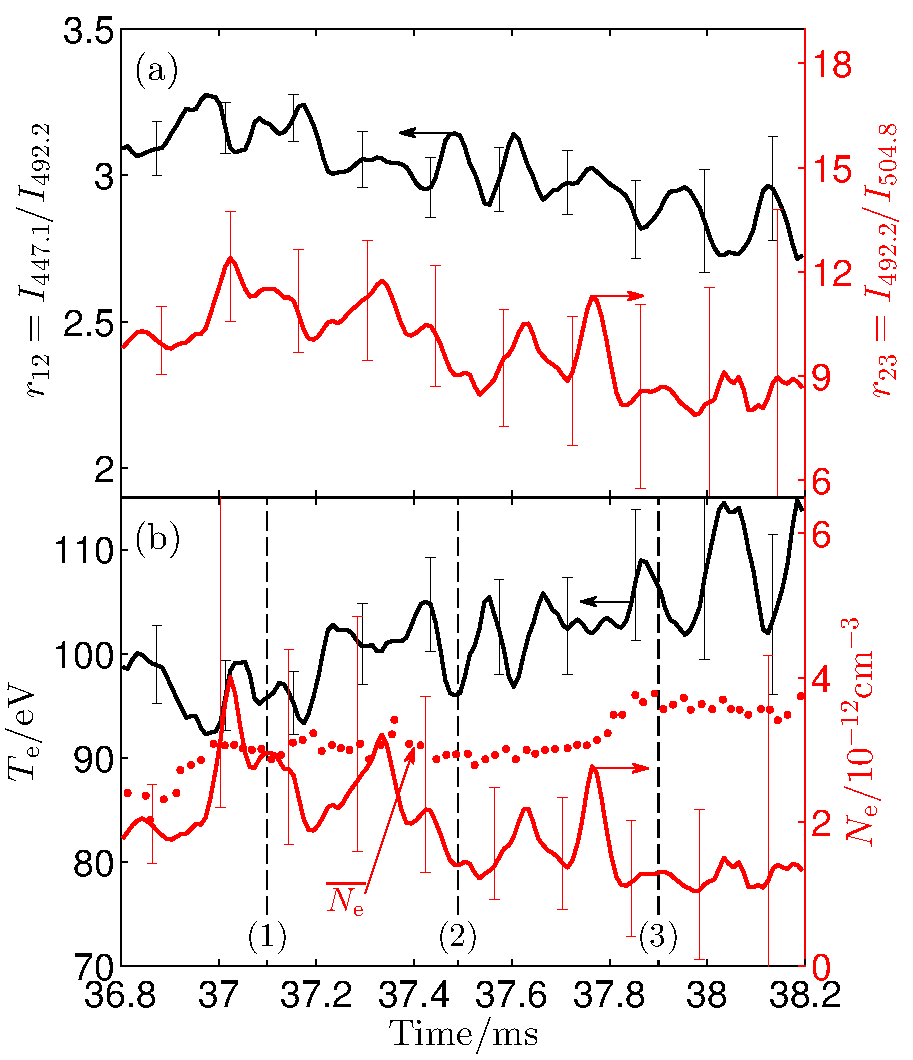
\includegraphics[height=0.9\textheight]{lineratio-te-ne-soliderrorbar}
  \end{figure}
\end{frame}

%\subsection{氦原子激发态数密度比较对模型结果的确认}
\subsection{碰撞辐射模型的复核}
\begin{frame}{激发态数密度:测量值与诊断所得参数下模型计算值}
	\centering
	\vspace{-0.5em}
    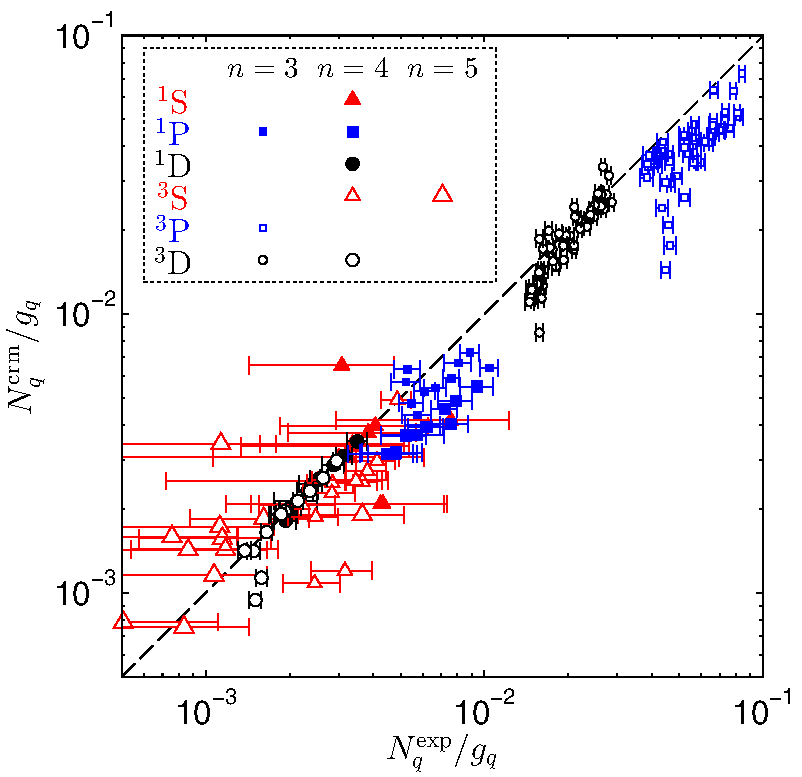
\includegraphics[height=0.9\textheight]{rel_levelabun-crm-to-exp}
\end{frame}

\subsection{光谱测量弦积分特性与谱线强度涨落的初步研究}

%\begin{frame}{谱线辐射强度分布}
%\end{frame}

\begin{frame}{谱线比与微波干涉仪测量的~$N_{\rm e}$ 与其空间分布的相关性}
        假设抛物线分布条件:
        $N_{\rm e}=N_{\rm e0}\left[1-(r/a)^2\right]^{\gamma_{N_{\rm e}}}$,
        $T_{\rm e}=T_{\rm e0}\left[1-(r/a)^2\right]^{\gamma_{T_{\rm e}}}$
    \vspace{-1em}
    \begin{columns}
    \column{0.5\textwidth}
        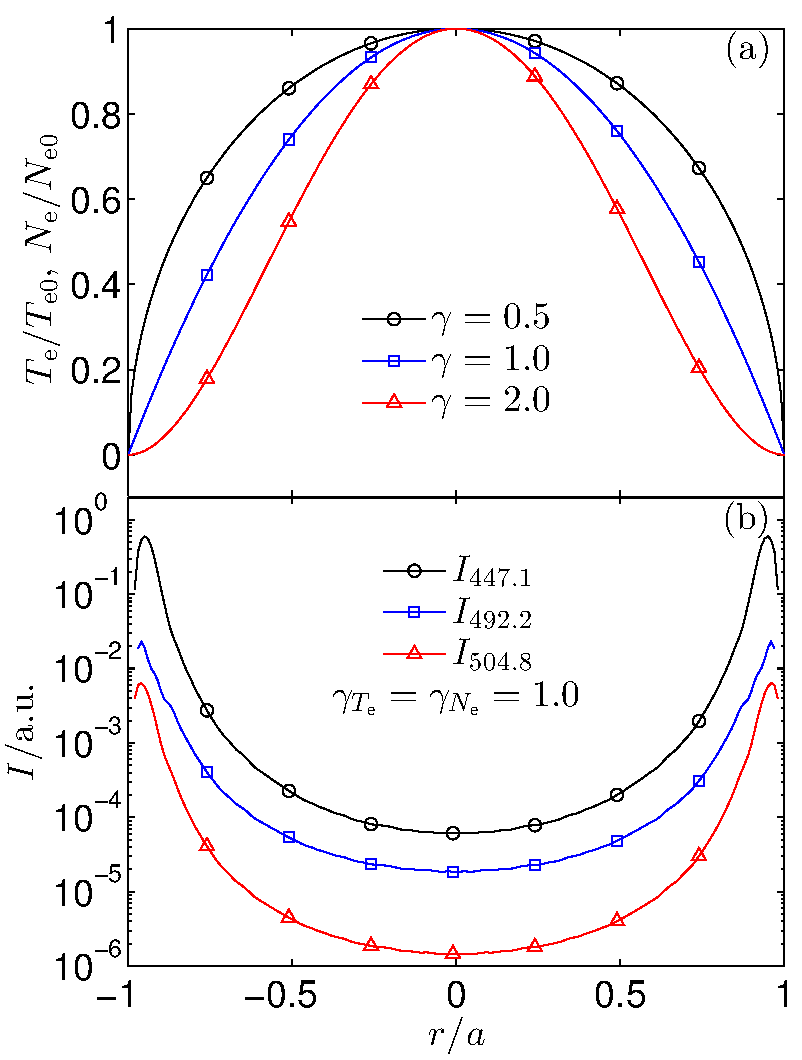
\includegraphics[width=0.9\textwidth]{ne-te-and-line-intensity-profile}
    \column{0.05\textwidth}
        \vspace{3cm}
        \color{red}{$\Longrightarrow$}
    \hspace{-0.05\textwidth}
    \column{0.5\textwidth}
    \begin{center}
        %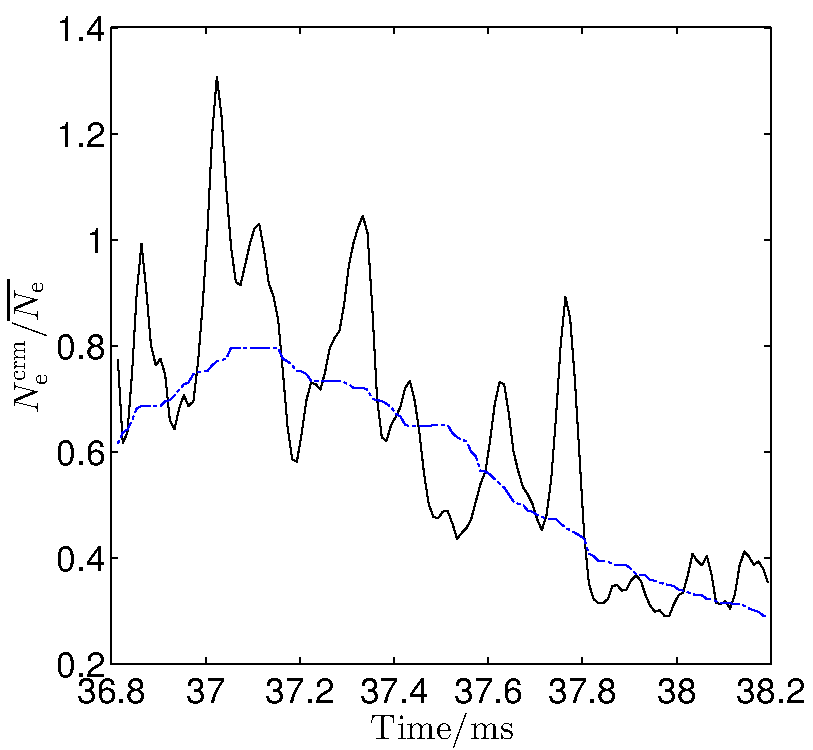
\includegraphics[height=0.4\textheight,width=0.9\textwidth]{ne-ratio-lineratio-to-mi}\\
        \begin{overpic}[height=0.4\textheight,width=0.9\textwidth]{ne-ratio-lineratio-to-mi}
        	\put(20,8.5){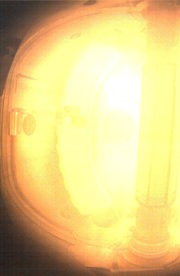
\includegraphics[width=0.12\textwidth]{he-plasama-shape-407}}
        	\put(25,30){$\uparrow$}
        	\put(50,40){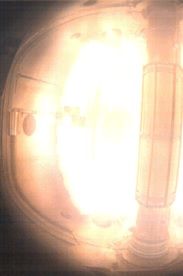
\includegraphics[width=0.12\textwidth]{he-plasama-shape-42}}
        	\put(55,35){$\downarrow$}
        	\put(75,25){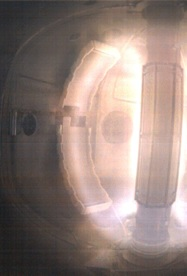
\includegraphics[width=0.12\textwidth]{he-plasama-shape-435}}
        	\put(80,20){$\downarrow$}
        \end{overpic}\\
        \vspace{-1.2em}
        \hspace{-2cm}\color{blue}{$\Updownarrow$}\\
        \vspace{-0.5em}
        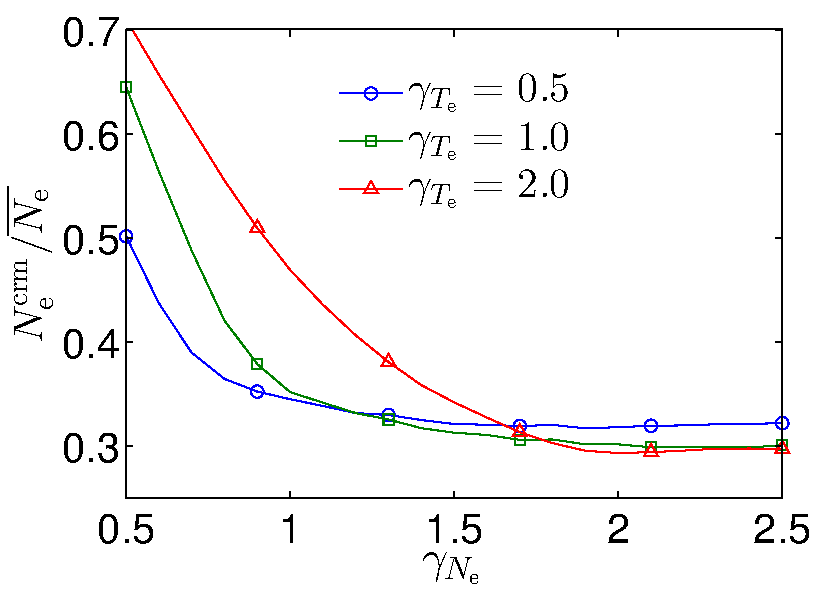
\includegraphics[width=0.9\textwidth]{line-int-ratio-params-to-mean-ne}
    \end{center}
    \end{columns}
\end{frame}

\begin{frame}{谱线涨落与磁探针信号涨落频谱分析}
	\vspace{-0.5em}
	\begin{figure}
      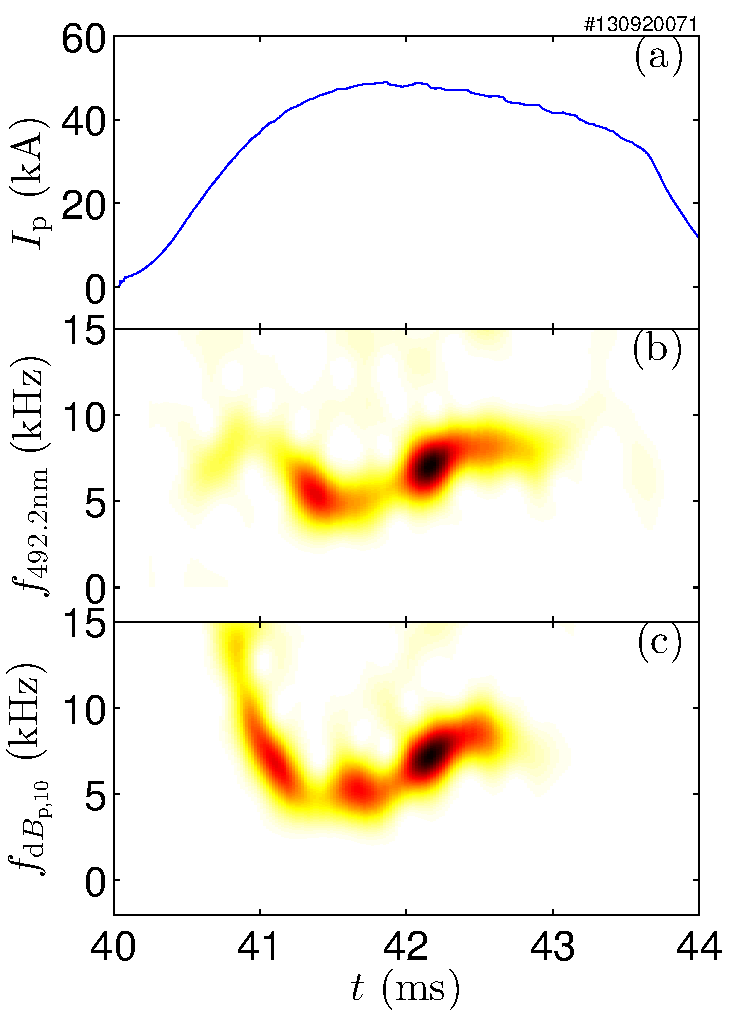
\includegraphics[height=0.9\textheight]{time_frequency_492_vs_dBp10}
  \end{figure}
\end{frame}

%\section{总结、创新点与研究的不足之处}
%\section{课题完成的工作内容、成果与不足之处}
\section{总结、课题主要创新与不足之处}

\begin{frame}{课题完成的工作内容与主要创新}
\definecolor{bulletcolor}{RGB}{0,0,160}
%\definecolor{bulletcolor}{RGB}{116,52,129}
	\begin{itemize}
		\item 课题完成的工作
			\begin{itemize}
				\item SUNIST 氦放电等离子体光谱诊断
					\begin{itemize}
						\item 碰撞辐射模型:适用于以下参数内,可忽略其他杂质影响的等离子体\\%包含能级数研究,速率系数不确定性传递函数推导
								{\footnotesize
								{\color{bulletcolor}\quad\tiny\raise1.5pt\hbox{{$\bullet$}}}~ $20{\rm eV}<T_e<300{\rm eV}$ \\
								{\color{bulletcolor}\quad\tiny\raise1.5pt\hbox{{$\bullet$}}}~ $1.0\times10^{12}{\rm cm}^{-3}<N_{\rm e}<2.0\times10^{13}{\rm cm}^{-3}$
								}
						\item 光谱诊断实验%:实验测量激发态能级验证模型
					\end{itemize}
%				\item SUNIST 上实验基础建设
			\end{itemize}
		\bigskip
		\item 课题主要创新
			\begin{itemize}
				\item 碰撞辐射模型方面
					\begin{itemize}
						\item 提出速率系数不确定性传递函数,可以对速率系数精度直接提出要求
						\item 给出结论:对具有 SUNIST 参数的等离子体碰撞模型,当 $\max n=7$ 时即给出可以接受的结果
						%模型中需包含的能级数
					\end{itemize}
				\item 实验方面
					\begin{itemize}
						%\item 为 SUNIST 建立了同时诊断 $T_{\rm e}$ 和 $N_{\rm e}$ 的手段
						\item 观察到以下结果\\
						{\footnotesize
							{\color{bulletcolor}\quad\tiny\raise1.5pt\hbox{{$\bullet$}}}~ 谱线比法与微波干涉仪测量的 $N_{\rm e}$ 之比与其分布峰化的相关性 \\
							{\color{bulletcolor}\quad\tiny\raise1.5pt\hbox{{$\bullet$}}}~ 光谱信号与磁探针信号具有一致的涨落行为
						}
%						\begin{itemize}
%							\item 谱线比法与微波干涉仪测量的弦平均电子密度之比与电子密度分布峰化的相关性
%							\item 光谱信号与磁探针信号具有一致的涨落行为
%						\end{itemize}
					\end{itemize}
%				\item SUNIST 实验基础方面
%					\begin{itemize}
%						\item 通过对脉冲进气特性研究,改善了 SUNIST 放电的重复性
%					\end{itemize}
			\end{itemize}
	\end{itemize}
\end{frame}

\begin{frame}{课题的不足之处与后续工作展望}
	\begin{itemize}
		\item 碰撞辐射模型的研究
			\begin{itemize}
				\item 不足:仅利用了模型的稳态解
				\item 后续工作:与实验结合,加入时变解,考虑非麦氏电子温度分布、能量粒子输运循环等因素,扩展适用范围至放电起始与结束阶段
%				\item 不足:仅在 SUNIST 上得到了验证
%				\item 后续工作:希望能在其他装置上进行实验验证并对模型进行改进和修正
			\end{itemize}
		\bigskip
		\item 光谱分析方面
			\begin{itemize}
				\item 不足:谱线展宽、波长位移诊断
				%\item 不足:测量无空间分辨
				\item 后续工作:建立新的实验设备,条件成熟时可以开展
			\end{itemize}
		\bigskip
		\item SUNIST 实验基础方面
			\begin{itemize}
				\item 不足:不具备空间分布诊断能力
				\item 后续工作:建立光电二极管阵列探测系统,结合断层反演技术以实现空间分辨诊断%新的实验设备,实现三条谱线的同时测量%,改进 SUNIST 基础放电状态
			\end{itemize}
	\end{itemize}
\end{frame}

\begin{frame}{课题论文发表情况}
	\small{
	\begin{itemize}
		\item SUNIST 上谱线比法的应用\\
			{\tiny Huiqiao Xie, Zhe Gao, Yi Tan, et al. Electron temperature and density determination in helium plasmas of SUNIST using the optical emission spectrum line-ratio method. The Joint Meeting of 5th IAEA Technical Meeting on Spherical Tori \& 16th International Workshop on Spherical Torus (\alert{ISTW2011}) \& 2011 US-Japan Workshop on ST Plasma, 2011: Toki}
		\item 实验基础建设:改善放电重复性\\
			{\tiny Xie Huiqiao, Tan Yi, Ke Rui, et al. Analysis of the gas puffng performance for improving the repeatability of Ohmic discharges in the SUNIST spherical tokamak. In press. (\alert{已被 Plasma Science and Technology 录用. SCI 源刊.})}
		\item 整体工作(包括了碰撞辐射模型中包含激发态能级数的研究等)\\
			{\tiny 谢会乔, 谭熠, 刘阳青, 等. SUNIST 氦放电等离子体的碰撞辐射模型及其在谱线比法诊断的应用. 物理学报, 2014 63(12): 125203. (\alert{SCI 源刊})} %(\alert{已被物理学报录用. SCI 源刊.})}
%		\item 碰撞辐射模型:速率系数不确定性误差传递函数\\
%			{\tiny Huiqiao Xie, Yi Tan, Yangqing Liu, et al. A new method for assessing the propagation of the uncertainties in excitation rate coefficients to the calculation of the helium collisional-radiative model(\alert{计划投稿})}
	\end{itemize}
	}
\end{frame}

\section{致谢}
\begin{frame}{致谢}
	\begin{itemize}
		\item 感谢高喆老师、蒲以康老师、王文浩老师、谭熠老师、解丽凤老师的教导、支持与鼓励
		\item 感谢王龙老师、杨宣宗老师和冯春华老师的关心爱护与帮助
		\item 感谢张良、曾龙、赵爱慧、刘阳青、姜艳铮、柴忪以及其他师兄弟姐妹的帮助与在实验室的陪伴
		\item 感谢工物系、西南物理研究院、等离子体所、工程物理研究院给予过帮助的所有老师和同学
		\item 感谢工作中在仪器制作、安装和调试中给过帮助的所有相关工程技术人员
		\item 感谢家人的爱护、支持与陪伴,尤其是张英女士
		\item 感谢学习生活中出现过的所有人士
		\item 深切怀念何也熙老师
	\end{itemize}
\end{frame}
%---- appendix ---- %
\appendix
%---- Thank you page ----%
\thankyoupage{感谢各位老师和同学出席!}

\backupframebegin

\begin{frame}{SUNIST 放电时静电探针烧蚀情况}
    \begin{center}
      \begin{overpic}[width=0.35\textwidth]{ProbeVapor121123020-bw.jpg}
    	\put(1,22){\color{white}{中心柱}}
    	\put(5,30){\color{white}{$\uparrow$}}
    	
    	\put(20,87){\color{white}{等离子体}}
    	\put(32,80){\color{white}{$\downarrow$}}
    	
    	\put(43,58){\color{white}{静电探针}}
    	\put(67,52){\color{white}{$\downarrow$}}
    	
    	\put(43,30){\color{white}{烧蚀亮点}}
    	\put(60,39){\color{white}{$\uparrow$}}
  	\end{overpic}
  		\\ SUNIST 静电探针烧蚀\\
  		\#121123020
  	\end{center}
\end{frame}

\begin{frame}{碰撞辐射模型对谱线比的预测:其他谱线比}
	\vspace{-0.3cm}
	\begin{center}
		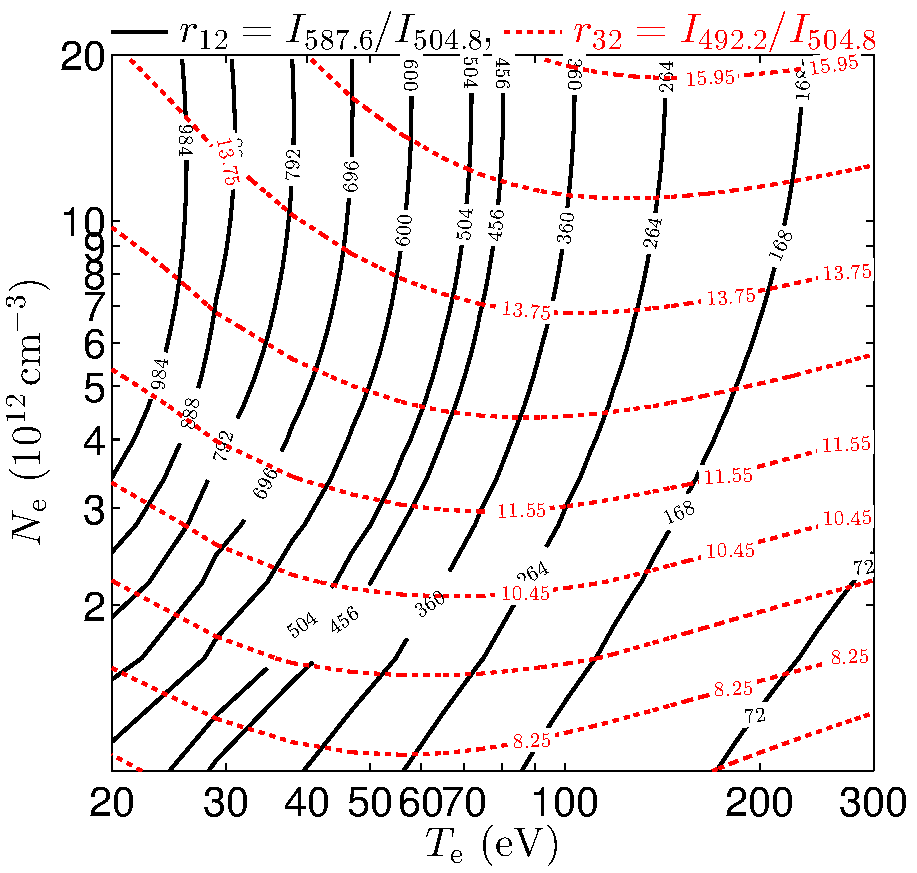
\includegraphics[height=0.9\textheight]{1-4to5-7to5-getTeNe-lineratio}
	\end{center}
\end{frame}

\begin{frame}{碰撞辐射模型对谱线比的预测:其他谱线比}
	\vspace{-0.3cm}
	\begin{center}
		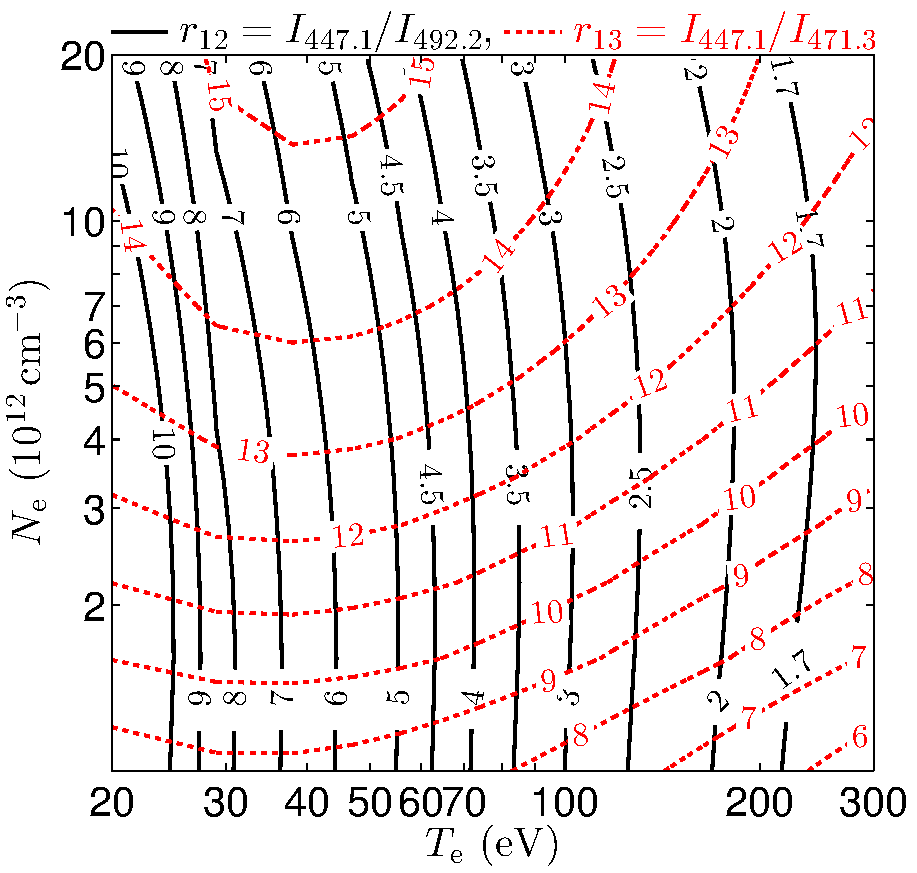
\includegraphics[height=0.9\textheight]{1-9to8-9to7-getTeNe-lineratio}
	\end{center}
\end{frame}

\begin{frame}{$N_{\rm e}$ and $T_{\rm e}$ Determination (6): Error Estimation Routes}
	\vspace{-0.3cm}
	\begin{center}
		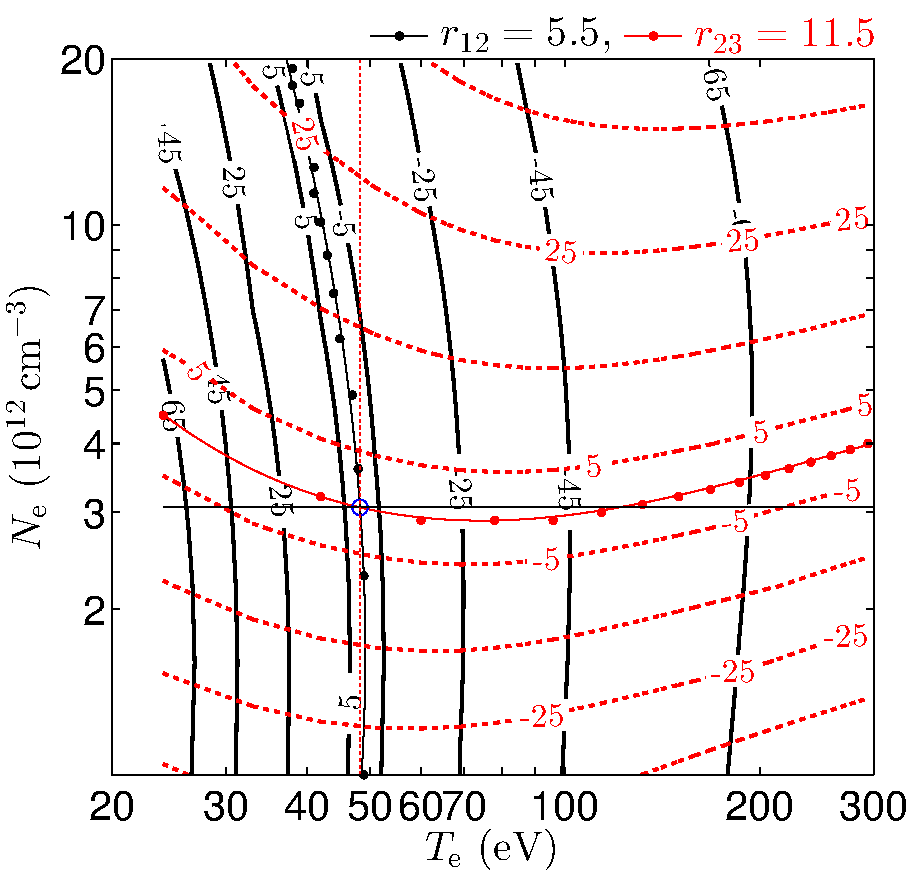
\includegraphics[height=0.9\textheight]{6-9to7-7to5-getTeNe-errorroute}
	\end{center}
\end{frame}

\begin{frame}{$N_{\rm e}$ and $T_{\rm e}$ Determination (7): Error Propagation}
	\vspace{-0.3cm}
	\begin{center}
		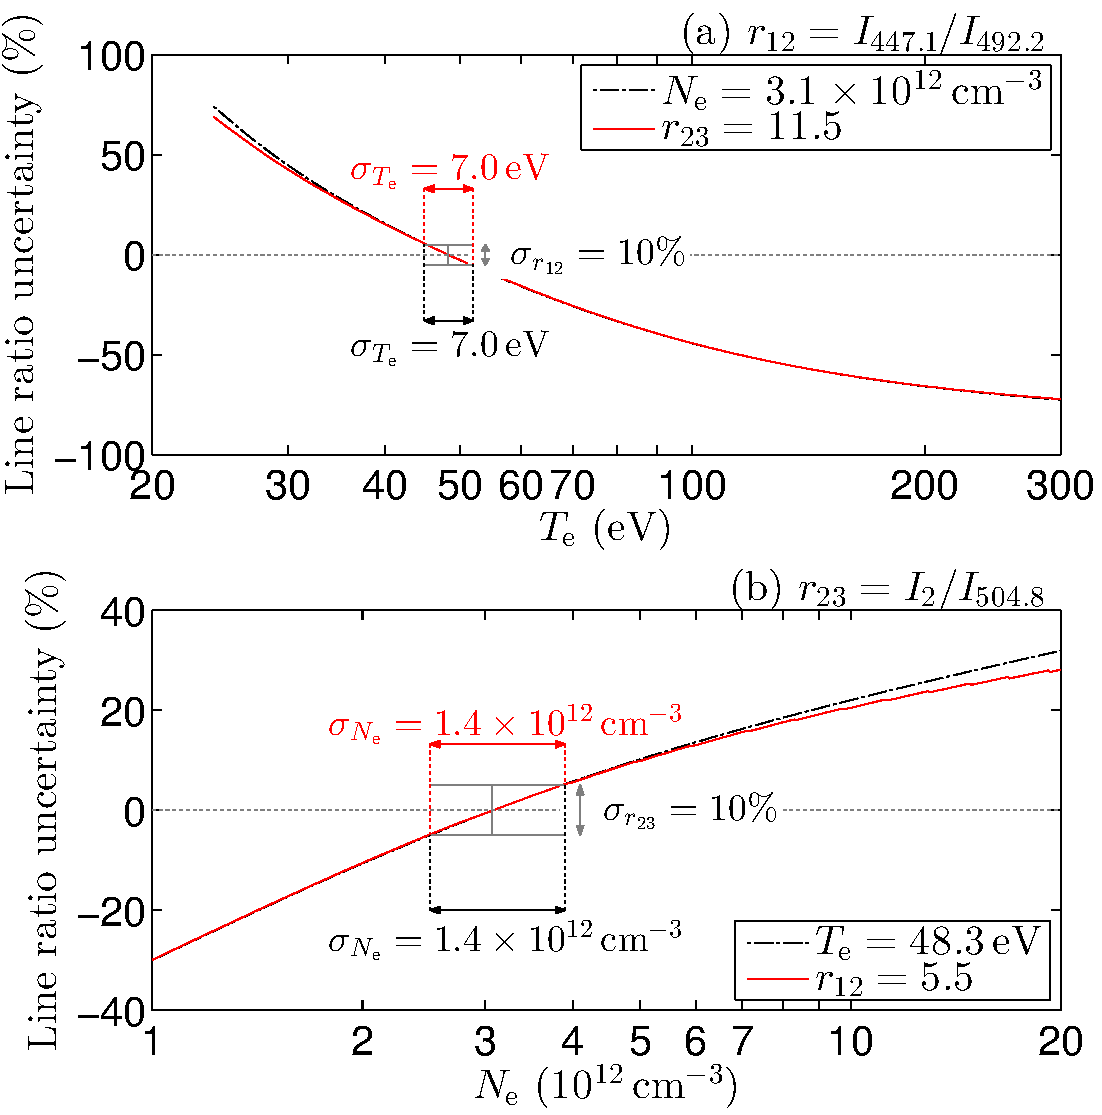
\includegraphics[height=0.9\textheight]{7-9to7-7to5-getTeNe-errorpropagation}
	\end{center}
\end{frame}

\begin{frame}{$N_{\rm e}$ and $T_{\rm e}$ Determination (8): Error Routes Comparison}
	\vspace{-0.3cm}
	\begin{center}
		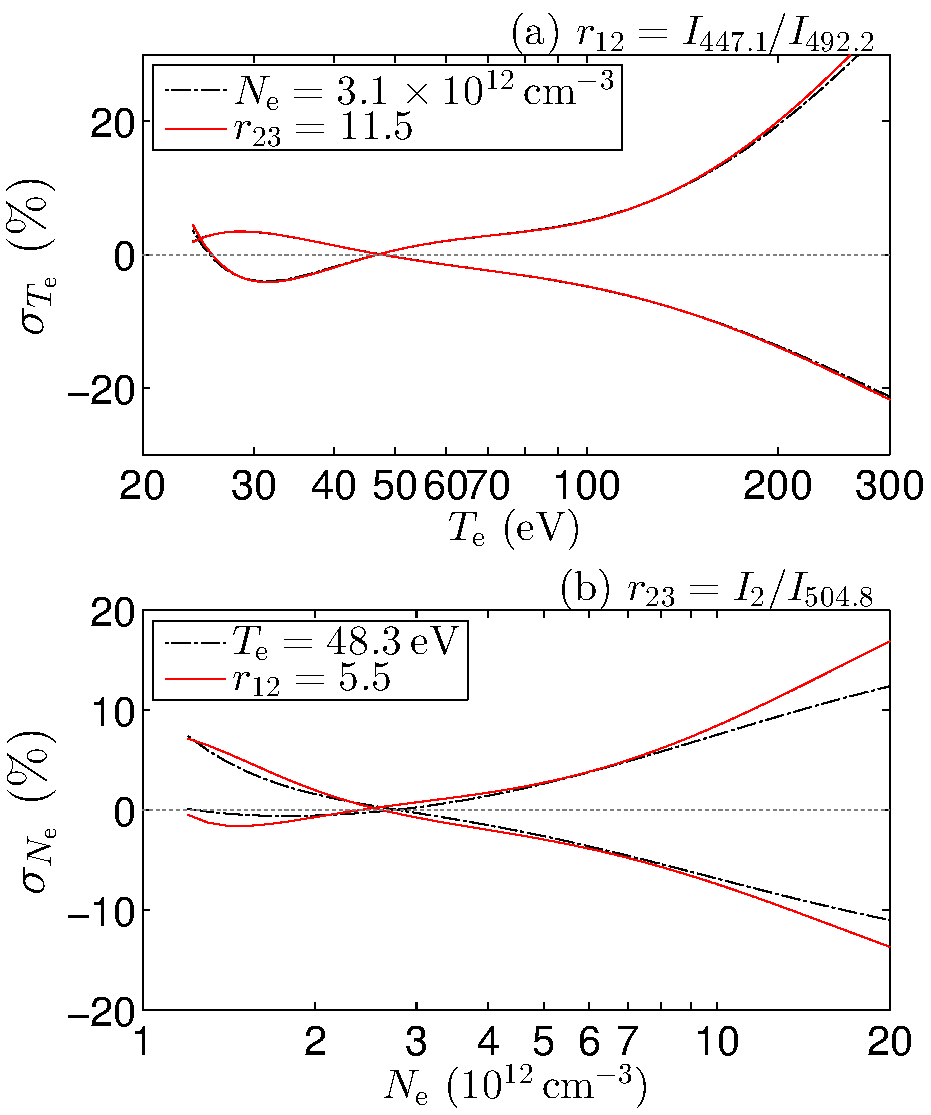
\includegraphics[height=0.9\textheight]{8-9to7-7to5-getTeNe-errorpropagationscan}
	\end{center}
\end{frame}


\begin{frame}{对谱线比计算结果的影响}
	\begin{itemize}
        \item 对谱线比计算结果的影响\onlineref{Burgos PoP (2012)}:
    \end{itemize}
    \begin{align*}
    \sigma_{r^{\rm mod}} \simeq & \pm r^{\rm mod} \\
    & \times\sqrt{2\left(\frac{\delta n}{n}\right)^2(1-\gamma_{qj})}
    \end{align*}

\end{frame}

\begin{frame}{实测:氦原子谱线比其他原子谱线强一个数量级以上}
	\centering
	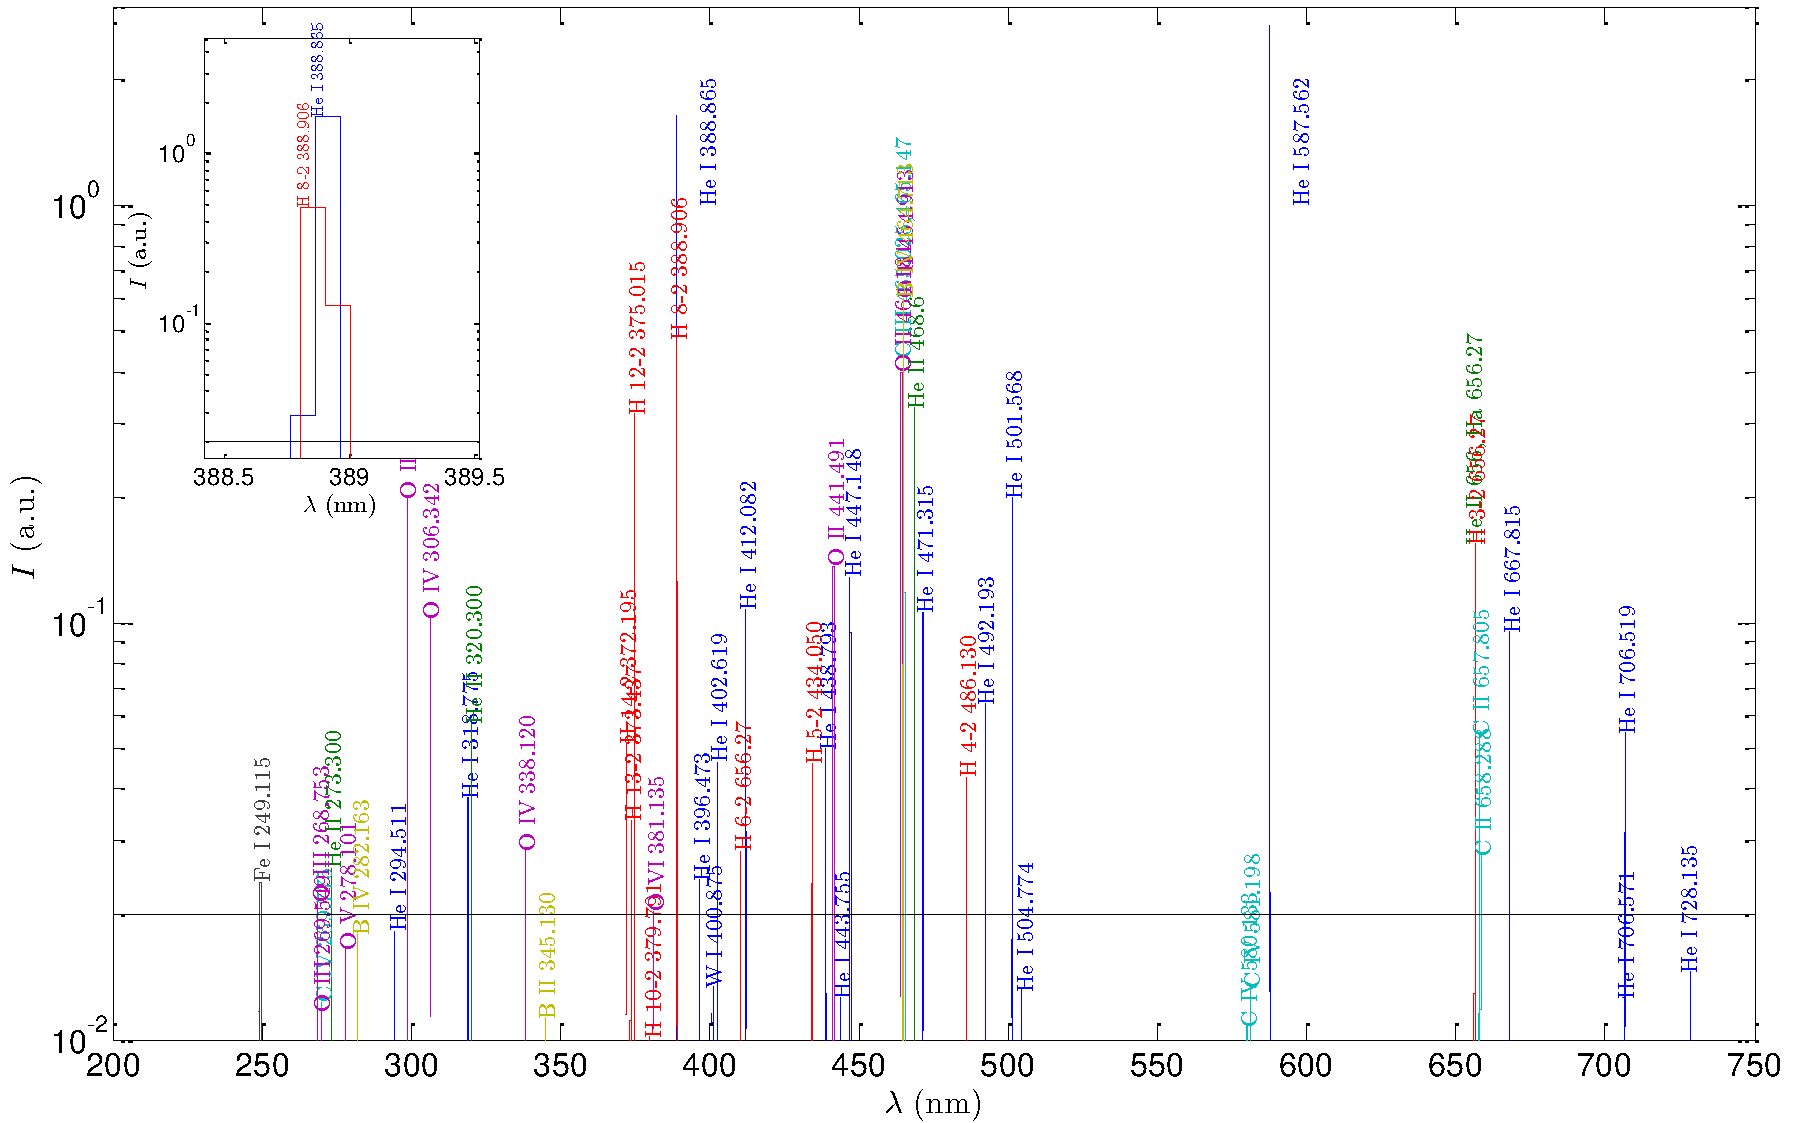
\includegraphics[width=\textwidth]{lines_in_he_plasma}
\end{frame}

\subsection{对 SUNIST 放电重复性的改善}

\begin{frame}{脉冲进气时真空室内气压分布变化规律}
	\centering
	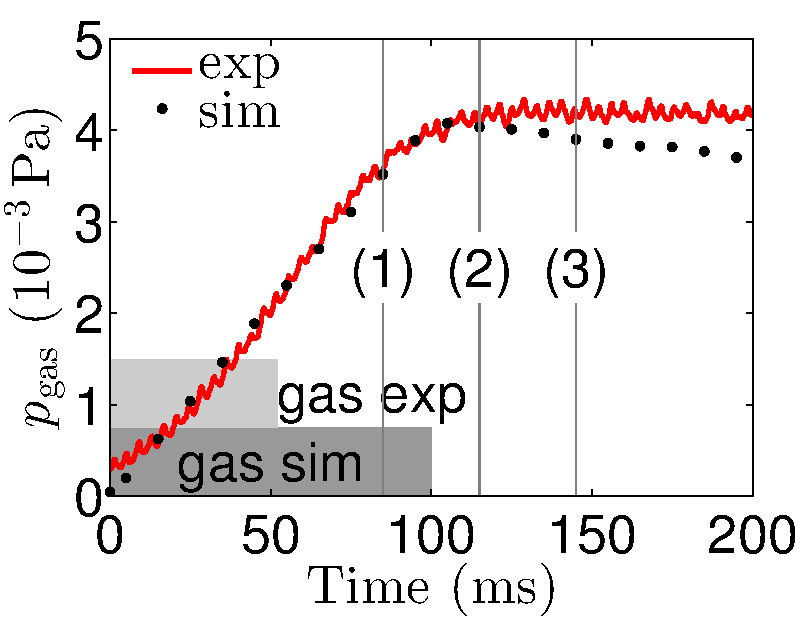
\includegraphics[height=0.45\textheight]{fig_6_a.pdf}\\
	\fbox{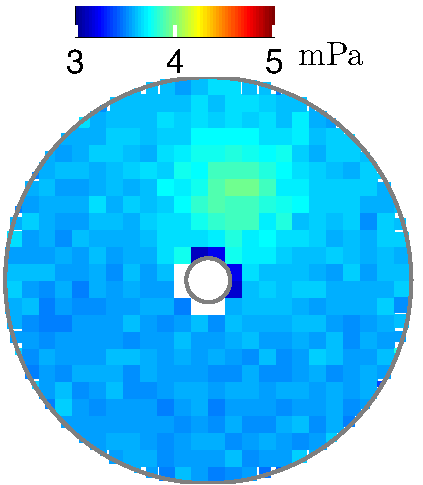
\includegraphics[height=0.4\textheight]{fig_6_b.pdf}}
	\fbox{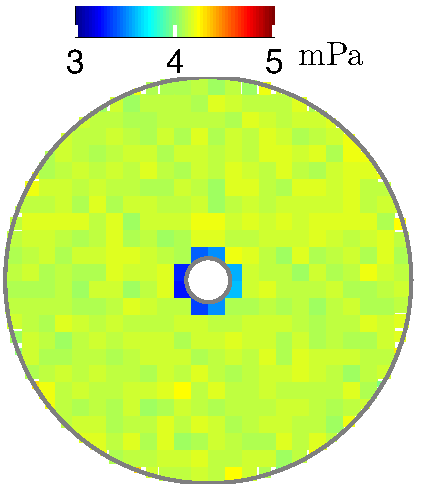
\includegraphics[height=0.4\textheight]{fig_6_c.pdf}}
	\fbox{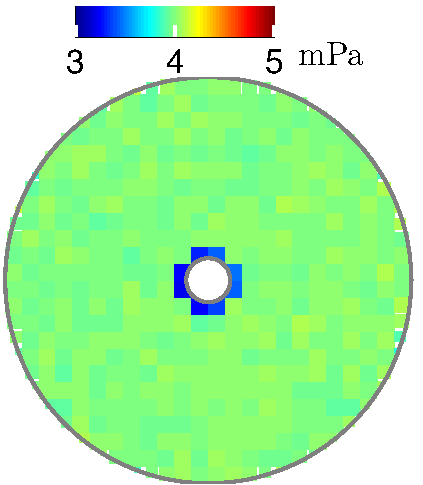
\includegraphics[height=0.4\textheight]{fig_6_d.pdf}}
\end{frame}

\begin{frame}{调整脉冲进气时序对放电重复性的改善}
	\centering
	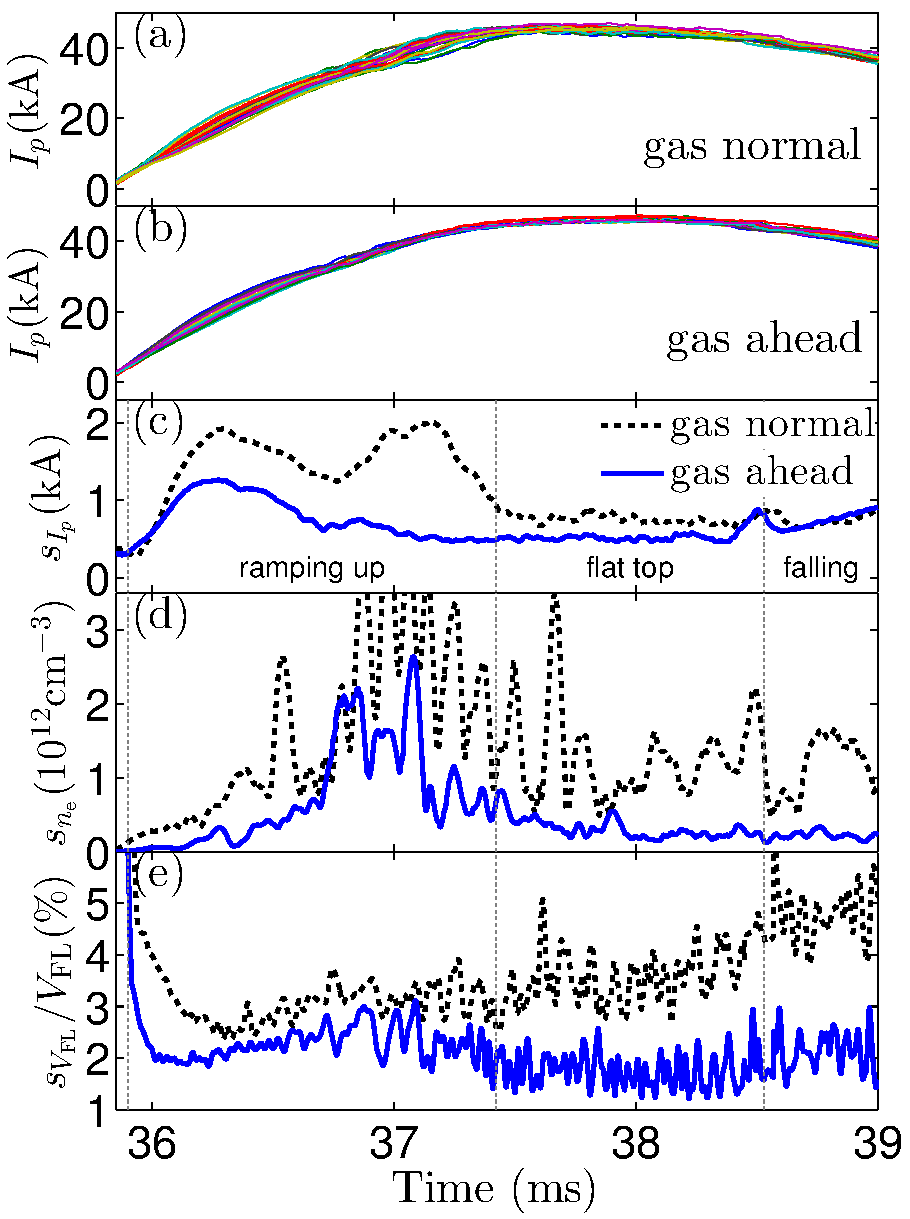
\includegraphics[height=0.9\textheight]{ip_vloop_ne_repeation_reacqdata}
\end{frame}

\subsection{SUNIST 上 $94\,{\rm GHz}$ 微波干涉仪}

%\begin{frame}{$94\,{\rm GHz}$ 微波干涉仪信号问题}
%	
%\end{frame}

\begin{frame}{微波干涉仪测量路径的确定}
	\begin{columns}
		\column{0.6\textwidth}
			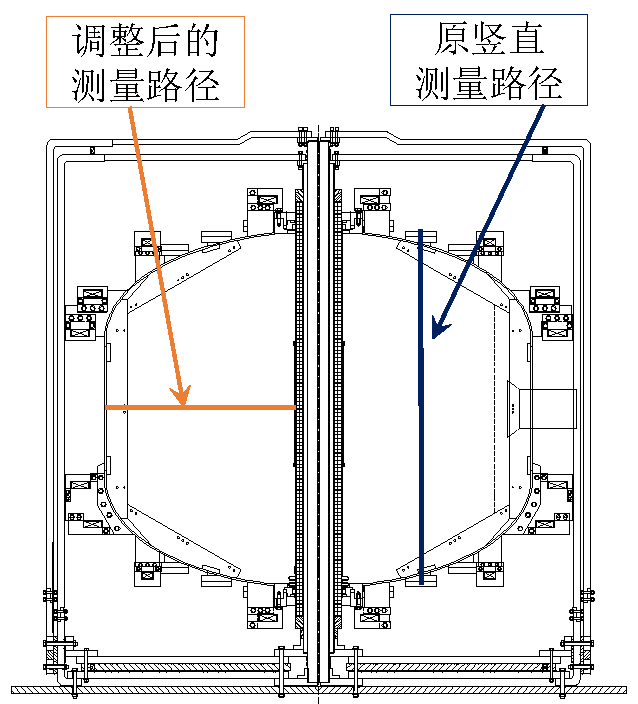
\includegraphics[height=0.8\textheight]{mi-route-both_cropped}
		\column{0.4\textwidth}
			\begin{overpic}[width=\textwidth]{ct-pt-before}
				\put(40,5){原竖直路径}
			\end{overpic}
			\\
			\begin{overpic}[width=\textwidth]{ct-pt-after}
				\put(43,5){水平路径}
			\end{overpic}
%			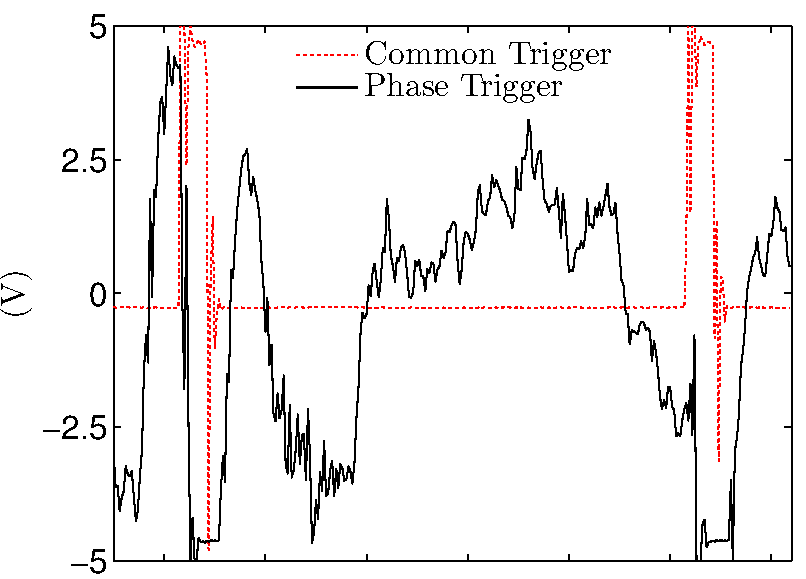
\includegraphics[width=\textwidth]{ct-pt-before}\\
%			\includegraphics[width=\textwidth]{ct-pt-after}
	\end{columns}
\end{frame}

\subsection{SUNIST 数据采集与处理服务系统}

\begin{frame}{SUNIST 数据采集与处理服务系统:目的与意义}
	\begin{itemize}
    \item 原有数据采集系统(WLYXZ)
    \begin{itemize}
      \item 采集通道数少:共32通道
      \item 软件环境不稳定(DOS@Windows98),容易丢失数据与宕机
      \item 数据管理与访问基于文件名
    \end{itemize}
    \bigskip%\pause
    \item SUNIST装置特性
    \begin{itemize}
      \item 实验数据量大,不断增加
      \item 每通道数据量随采集时间、频率等变化
      \item 实验人员频频繁访问处理数据
    \end{itemize}
    \bigskip%\pause
    \item 新的数据采集与处理服务系统
    \begin{itemize}
      \item 信号采集能力升级,与SUNIST升级后众多诊断设备整合匹配
      \item 基于炮号管理数据,系统软件环境稳定
      \item 分布式访问数据,提供多种编程接口,多人协作参与实验能力
    \end{itemize}
  \end{itemize}
\end{frame}

\begin{frame}{升级后的 SUNIST 数据采集与处理服务系统(SDSup)}
  \centering
  \alert{S}UNIST \alert{D}ata acquisition and processing \alert{S}erving system \alert{Up}grade
  \begin{figure}
      \includegraphics[width=\textwidth]{data-system-chs_cropped}
  \end{figure}
\end{frame}

\begin{frame}{Time Constants}
	%\centering
	\begin{description}
		\item[intrinsic group]
			$\tau_a\sim 10^{-13}\rm{s}\,{<<}\,
				\tau_o\sim \frac{10^{-8}}{z^4}\rm{s}\,{<<}\,
				\tau_m\sim \frac{10^{1}}{z^8}\rm{s}$
		\item[extrinsic group]
			$\tau_{\rm{ion, rec}}>>\tau_{\rm{i-e}}>>\tau_{\rm{i-i}}>>\tau_{\rm{e-e}}$
		\item[to be compared with $\tau_{\rm{plasma}}$]
			$\tau_{\rm{plasma}}\sim\tau_{g}\sim\tau_{m}>>\tau_{o}>>\tau_{\rm{e-e}}$
	\end{description}
	\begin{itemize}
		\item quasi-equilibrium:
			\begin{itemize}
				\item partially de-coupled from transport problem - local calculation
				\item metstable, ground level, ions are the dominant populations
			\end{itemize}
	\end{itemize}
\end{frame}

\begin{frame}{Plasma Conditions of Helium Discharges}
	\begin{itemize}
		\item $T_e$: $\sim 200\rm{eV}$, $N_e$: $5\times 10^{12}-3\times 10^{13}\rm{cm}^{-3}$
			%\footnote{W H Wang {\it\footnotesize et al.} PPCF (2005) {\bf\footnotesize 47} 1-16}
		\item Particle species: $\rm{He}$ atom, $\rm{He}^+$, $\rm{He}^{+2}$, $\rm{H}_2$, $\rm{H}$ atom, $\rm{H}^+$
		\item Reactions:
			\begin{itemize}
				\item neutral atom: excitation, deexcitation, ionization, double ionization
				\item $\rm{He}^+$: ionization, recombination
				\item $\rm{He}^{+2}$: recombination
				\item $\rm{H}_2$: $\rm{e}+\rm{H}_2\leftrightharpoons\rm{H}^*+\rm{H}+\rm{e}$,
					$\rm{He}^*+\rm{H}_2\leftrightharpoons\rm{H}^*+\rm{He}+\rm{H}$
				\item $\rm{H}$: $\rm{e}+\rm{H}\leftrightharpoons\rm{H}^*+\rm{e}$,
					$\rm{e}+\rm{H}\leftrightharpoons\rm{H}^++\rm{e}$,
					$\rm{He}^{\rm meta}+\rm{H}^+\leftrightharpoons\rm{H}+\rm{He}^+$
			\end{itemize}
        \item the pure He CR model (without H)
            \begin{itemize}
              \item the main H and He reactions: $\rm{He}^{\rm meta}+\rm{H}^+\leftrightharpoons\rm{H}+\rm{He}^+$
              \item the population densities of meta-stables are far small compared to $gs$ and the ions
              \item the fractional content of H is small (RGA results)
            \end{itemize}
	\end{itemize}
\end{frame}

\begin{frame}{the Uncertainty Propagation Analysis}
	%\vspace{-0.5em}
	\begin{itemize}
        %\item the uncertainties of the rates between the same $n$ and those from $hl$ dominate the error in population densities of the excited states
		\item Based on the analysis of $n=3$ states
        %\item $\sigma_{N_p}=E_{jp}\sigma_{C_{jp}}\simeq2\frac{f_{jp}}{F_{p,in}}\sigma_{C_{jp}}$
	\end{itemize}
	\vspace{-2em}
	\begin{columns}
			\column{0.33\textwidth}
				\includegraphics[width=\textwidth]{transfer-n3-Brenning}\\
				\mbox{\tiny [\texttt{N. Brenning J.Phys.D (1980)}]}
			\column{0.02\textwidth}
				$\Rightarrow$
			\column{0.25\textwidth}
				\vspace{2.5cm}
				\includegraphics[width=\textwidth]{exc_rates_error_cropped}\\
				\vspace{2.1cm}
				\mbox{{\tiny [\texttt{Y Andrew PPCF(2000)}]}$\to$}
			\column{0.02\textwidth}
				$\Rightarrow$
			\column{0.38\textwidth}
				\includegraphics[height=0.9\textheight]{fractional_change_31S_cropped}
	\end{columns}
	
\end{frame}


\begin{frame}{deducing the Uncertainty Propagation Function of the uncertainties in the rate coefficients}
    \vspace{-0.5em}
    \begin{center}
        \includegraphics[width=\textwidth]{deducing-the-uncertainty-prop-fun}
    \end{center}
\end{frame}

\begin{frame}{tomography measurements and the future plan (1)}
    \vspace{-0.5em}
    \begin{center}
        \includegraphics[width=\textwidth]{tomography-plan-illustration}
    \end{center}
\end{frame}

\begin{frame}{tomography measurements and the future plan (2)}
    \vspace{-0.5em}
    \begin{center}
        \includegraphics[width=0.453\textwidth]{chords_conf}
        \includegraphics[width=0.547\textwidth]{pinholescan}
    \end{center}
\end{frame}

\begin{frame}{tomography measurements and the future plan (3)}
    \vspace{-0.5em}
    \begin{center}
        \includegraphics[height=0.9\textheight]{testplot}
    \end{center}
\end{frame}

\begin{frame}{the Line shape analysis and $T_i$ diagnostics (1)}
    \begin{columns}
      \column{0.6\textwidth}
      \centering
      \begin{itemize}
        \item FWHM estimation of the lines (right)
        \item Monochromator: resolution~0.2 \AA%, 步长~0.05 \AA
        \item For He ~501.568 nm:
            \includegraphics[width=0.9\textwidth]{line-shape-gen-demo}
        %\item 后续工作:
%            \begin{itemize}
%              \item 斯塔克展宽与赛曼分裂的考虑
%              \item 使用更高分辨率扫描谱线
%            \end{itemize}
      \end{itemize}

      \column{0.4\textwidth}
      \begin{center}
        \includegraphics[width=\textwidth]{lineshape-parameters}\\
		\includegraphics[width=\textwidth]{lineshape-estimates}
      \end{center}
    \end{columns}
\end{frame}

\begin{frame}{the Line shape analysis and $T_i$ diagnostics (2)}
    \vspace{-0.5em}
    \begin{center}
        \includegraphics[height=0.9\textheight]{he-line-ratio-and-ne-te-fwhm-ti}
    \end{center}
\end{frame}

\begin{frame}{速率系数不确定性:各能级的主要产生过程}
	\centering
	\includegraphics[height=0.8\textheight]{Ne1E12_Te300_1e7cm-3s-1}
\end{frame}

\begin{frame}{速率系数不确定性:各能级的主要产生过程}
	\centering
	\includegraphics[height=0.8\textheight]{Ne1E13_Te30_1e7cm-3s-1}
\end{frame}

\begin{frame}{速率系数不确定性:各能级的主要产生过程}
	\centering
	\includegraphics[height=0.8\textheight]{Ne1E13_Te300_1e7cm-3s-1}
\end{frame}

\begin{frame}{忽略氢与其他杂质的影响:含量低、截面小}
	\begin{itemize}
		\item 杂质粒子中氢的含量最高%真空室本底 ${\rm H}_2{\rm O}$ 和 ${\rm H}_2$ 较难去除
		\begin{itemize}
			\item 本底质谱:等效 ${\rm H }\sim 40\% @ 1\times10^{-4}{\rm Pa}$~|~氦放电气压 $4.3\times10^{-3}{\rm Pa}$
%			\item 氦放电气压 $4.3\times10^{-3}{\rm Pa}$
			\item 电子与质子碰撞激发与电离截面的对比:
		\end{itemize}
	\begin{columns}
		\column{0.5\textwidth}
			\centering
			\begin{overpic}[width=\textwidth]{he-exc-xsec-compare}
				\put(20,62){电子与质子碰撞激发截面}
			\end{overpic}
		\column{0.5\textwidth}
			\centering
			\begin{overpic}[width=\textwidth]{he-ionization-xsec-comapre}
				\put(20,62){电子与质子碰撞电离截面}
			\end{overpic}
	\end{columns}
		\onlineref{Anderson H PhD Thesis(1999)}
		\bigskip
		\item 其他 C、N、O 等杂质含量不会高于 H\onlineref{RC Isler NF(1984)}%比 ${\rm H}$ 低
	\end{itemize}
\end{frame}


\begin{frame}{碰撞辐射模型中考虑的主要粒子、反应过程}
%	\begin{columns}
%	\column{0.4\textwidth}
	\begin{itemize}
		\item 考虑的粒子
		\begin{itemize}
			\item ${\rm e}$、${\rm He}(n^{2S+1}L)$、${\rm He}^+$、${\rm He}^{2+}$
		\end{itemize}
		\bigskip
		\item 考虑的反应过程
		\begin{itemize}
			\item 电子碰撞激发/退激发
			\item 电子碰撞电离/复合
			\item 自发辐射跃迁
		\end{itemize}
	\end{itemize}
%	\column{0.6\textwidth}
%\begin{center}{\tiny
%\begin{tabular}{ccc}\toprule
%跃迁 & \makecell[c]{$\lambda_{q\to p}$\\ (${\rm nm})$} & \makecell[c]{$A_{q\to p}^{\rm eff}$\\ ($10^7\,{\rm s}^{-1}$)}\\
%\hline
%$2^1{\rm S}\leftarrow3^1{\rm P}$ & 501.6 & 1.34 \\
%$2^1{\rm S}\leftarrow4^1{\rm P}$ & 396.5 & 0.70 \\
%$2^1{\rm P}\leftarrow4^1{\rm S}$ & 504.8 & 0.68 \\
%$2^1{\rm P}\leftarrow4^1{\rm D}$ & 492.2 & 1.99 \\
%$2^3{\rm S}\leftarrow3^3{\rm P}$ & 388.9 & 0.95 \\
%$2^3{\rm P}\leftarrow3^3{\rm D}$ & 587.6 & 7.07 \\
%$2^3{\rm P}\leftarrow4^3{\rm S}$ & 471.3 & 0.95 \\
%$2^3{\rm P}\leftarrow4^3{\rm D}$ & 447.1 & 2.46 \\
%$2^3{\rm P}\leftarrow5^3{\rm S}$ & 412.1 & 0.45 \\
%\bottomrule
%\end{tabular}
%}
%\includegraphics[width=0.33\textwidth]{1-9to7-7to5-getTeNe-lineratio}
%\includegraphics[width=0.33\textwidth]{1-4to5-7to5-getTeNe-lineratio}
%\includegraphics[width=0.33\textwidth]{1-9to8-9to7-getTeNe-lineratio}
%\end{center}
%	\end{columns}
\end{frame}

\backupframeend

\end{CJK*}
\end{document}
